% -*- phrases: HW2 -*-
\documentclass[pdftex,11pt]{article}
\usepackage[utf8]{inputenc}
\usepackage{tikz}	
\usepackage{graphicx}
\usepackage{listings}
\usepackage{color}
\usepackage{layout}
\usepackage{pdflscape}
\usepackage{hyperref}
\usepackage{appendix}
\usepackage{pdfpages}

\hypersetup{colorlinks=true, linkcolor=blue, citecolor=blue, filecolor=blue, urlcolor=blue, pdftitle=Capstone Portfolio: Drone Flight Planning Software, pdfauthor=David Klingenberg, pdfsubject=, pdfkeywords=}

\DeclareGraphicsExtensions{.pdf,.png,.jpg}

\marginparwidth = 0pt
\marginparsep = 0pt
\topmargin = 0pt
\oddsidemargin = 0pt
\textwidth = 468pt
\textheight = 581pt
\lstset{
  language=C,                     % choose the language of the code
  numbers=left,                   % where to put the line-numbers
  stepnumber=1,                   % the step between two line-numbers.        
  numbersep=5pt,                  % how far the line-numbers are from the code
  backgroundcolor=\color{white},  % choose the background color. You must add \usepackage{color}
  showspaces=false,               % show spaces adding particular underscores
  showstringspaces=false,         % underline spaces within strings
  showtabs=false,                 % show tabs within strings adding particular underscores
  tabsize=2,                      % sets default tabsize to 2 spaces
  captionpos=b,                   % sets the caption-position to bottom
  breaklines=true,                % sets automatic line breaking
  breakatwhitespace=true,         % sets if automatic breaks should only happen at whitespace
  title=\lstname,                 % show the filename of files included with \lstinputlisting;
}

 
\newcommand{\HRule}{\rule{\linewidth}{0.5mm}}

\begin{document}
\pagenumbering{gobble}
\begin{titlepage}

\begin{titlepage}
\begin{center}

% Upper part of the page. The '~' is needed because \\
% only works if a paragraph has started.

\includegraphics[width=0.15\textwidth]{./icons/04UI_Seal-Black.jpg}~\\[1cm]

\textsc{\LARGE University of Idaho}\\[1.5cm]

\textsc{\Large CS 270}\\[0.5cm]

% Title
\HRule \\[0.4cm]
{ \huge \bfseries Capstone Portfolio \\[0.4cm] }
{ \huge \bfseries Drone Mission Planning Software \\[0.4cm] }
\HRule \\[1.5cm]
\centerline{\emph{Team:}}
\centerline{Mission Control}
% Author and supervisor
\noindent
\begin{minipage}{0.4\textwidth}
\begin{flushleft} \large
\emph{Authors:}\\
David \textsc{Klingenberg}\\
Taylor \textsc{Trabun}
\end{flushleft}
\end{minipage}%
\begin{minipage}{0.4\textwidth}
\begin{flushright} \large
\vspace{20pt}
\emph{Advisors:} \\
Dr.~Bruce \textsc{Bolden}\\
Dr.~Robert \textsc{Rinker}\\
\vspace{10pt}
\emph{Customer:}\\
Brandon \textsc{Ortiz}
\end{flushright}
\end{minipage}

\vfill

% Bottom of the page
{\large \today}

\end{center}
\end{titlepage}
\newpage
\thispagestyle{empty}
\mbox{}
\end{titlepage}

\tableofcontents
\listoffigures
\listoftables

\clearpage
\pagenumbering{arabic}
\setcounter{page}{1}
\section{Team Member Contact Information}
  	\begin{table}[h]
  	\centering
		\begin{tabular}{| l | c | p{5cm} |}
		\hline
		Name & Phone Number & Email Address\\\hline
		Joseph Higley & & higley@vandals.uidaho.edu\\
		David Klingenberg  &  (208) 310-9657 &  bigwookiee@Gmail.com\\
		Emeth Thompson & & thom5468@vandals.uidaho.edu\\
		Taylor Trabun & (509) 995-0904 & trab1744@vandals.uidaho.edu\\
		\hline
	\end{tabular}
\caption{Team Member Contact Information}
\label{table:1}
\end{table}


\section{Introduction}


Software to create and upload a flight plan to a quad copter drone. The flight plan will be uploaded using xBee radio communication.\\

This project will use off-the-shelf parts.  ATMEL\textsuperscript{\textcopyright} based microcontrollers found on ardunio based open source boards is the current preference.

\subsection{Target Priorities}

\begin{table}[h]
	\centering
	\begin{tabular}{c | c | p{8cm} | c}
	\hline
		 Number & Category & Need & Importance \\ \hline
		 1 & Quadcopter & Center of Gravity Refined & 5 \\
		 2 & Quadcopter & Reliable Flight & 5 \\
		 3 & Quadcopter & Functioning xBee Hardware &  4 \\
		 4 & Quadcopter & Hardware (Microcontroller) with xAPI and services to control flight & 5 \\
		 5 & Quadcopter & Controlled with XP communications &  4 \\
	   6 & Quadcopter & Autoland & 5 \\
	   7 & Software & software package for flight planning & 2\\
	   8 & Software & API for sending commands from computer & 2\\
	\end{tabular}
	\caption{Priorities}
	\label{table:2}
\end{table}

\clearpage
\section{Initial Client Interview Transcript 9/10/14}
\label{sec:clienttranscript}
%\documentclass[11pt,a4paper]{article}
%\usepackage[utf8]{inputenc}
%\usepackage{amsmath}
%\usepackage{amsfonts}
%\usepackage{amssymb}
%\title{Client Interview Transcript 9/10/14}
%\author{Team: Mission Control; Taylor Trabun and David Klingenberg}
%\begin{document}
%
%\textbf{Team: Mission Control; Taylor Trabun and David Klingenberg}
\textbf{Mentor/Client: }Brandon Ortiz

\subsection{Meetings}
We will be having weekly meetings in Brandon's office on Thursdays at 3:30 PM. These meeting will include status updates, further work on designs, troubleshooting, and assignment of tasks

\subsection{End Goal}
To have a stable and flying quadcopter that can be communicated with remotely. In addition, work done on a flight planning software (including GUI) should be underway. The project will be done in small steps, as this project requires research and development throughout.

\subsection{First Steps}
	\begin{itemize}
		\item Learn how quadcopter works
		\item Reconstruct quadcopter to be stable 
		\item Learn how to fly quadcopter
		\item Understand flight computer documentation
		\item Design communications
		\item Be sure to use xAPI
	\end{itemize}
	
\subsection{Requirements}
	\begin{itemize}
		\item Functional quadcopter (stable)
		\item Documentation of quadcopter construction
		\item Use of xAPI on arduino communication system
		\item Communication system using xBEE to communicate from computer to quadcopter
		\item Ability to send commands to quadcopter
		\item Flight planning software, including GUI
	\end{itemize}
	
\subsection{Other Notes}
Other notes from the meeting included aviation terminology, how to pair the remote control and quadcopter receiver, quick tour of controller and motor adjustments, and a quick tour of flight computer.
%\end{document}
\clearpage


\section{Meeting Agendas}
%\addcontentsline{toc}{section}{Agendas}
%\addtocounter{section}{1}

% Agenda %%%%%%%%%%%%%%%%%%%%%%%%%%%%%%%%%%%%%%%%%%%%%%%%%%%%%%%%%%%%%%%%%%%%%%%%
\subsection{Sept. 10, 2014}
{ \huge \bfseries Mission Control Team Agenda \\[0.4cm] }
{ \huge \bfseries Friday September  10, 2014.\\1500 –-  1600  in JEB   Think  Tank. \\[0.4cm] }
\vspace*{2.5mm}

{ \large \bfseries \hspace*{2 mm} Type of Meeting\\}
\hspace*{12 mm} Initial client interview.
\vspace*{1.5mm}

{ \large \bfseries \hspace*{2 mm} Attendees\\}
\hspace*{12mm} David Klingenberg\\
\hspace*{12mm} Taylor Trabun\\
\hspace*{12mm} Brandon Ortiz\\
\vspace*{1.5mm}

{ \large \bfseries \noindent Topics}
\vspace*{2.5mm}

\begin{tabular}{| l | l | l |}
  \hline
  \bfseries Topic & \bfseries Responsible & \bfseries Time (in minutes) \\ \hline
  Product  Overview  &  Brandon &  15 \\ \hline
  System  Requirements & Brandon & 15 \\ \hline
  Tasks Breakdown & Open Discussion & 15 \\ \hline
  Question \&  Answers  & Open Discussion & 25 \\ 
  \hline
\end{tabular}

\vspace*{2.5mm}
{ \large \bfseries \noindent Additional Information:}
This is our initial client interview.

\subsubsection[short]{Minutes from Friday September 10 Meeting}
Refer to \hyperref[sec:clienttranscript]{Section~\ref{sec:clienttranscript}} initial client  transcript.

% Agenda %%%%%%%%%%%%%%%%%%%%%%%%%%%%%%%%%%%%%%%%%%%%%%%%%%%%%%%%%%%%%%%%%%%%%%%%%%

\subsection{Sept. 18, 2014}
{ \huge \bfseries Mission Control Team Agenda \\[0.4cm] }
{ \huge \bfseries Thrusday September  18, 2014.\\1500 –-  1600  in JEB   Think  Tank. \\[0.4cm] }
\vspace*{2.5mm}

{ \large \bfseries \hspace*{2 mm} Type of Meeting\\}
\hspace*{12 mm} Initial Planning
\vspace*{1.5mm}

{ \large \bfseries \hspace*{2 mm} Attendees\\}
\hspace*{12mm} David Klingenberg\\
\hspace*{12mm} Taylor Trabun\\
\hspace*{12mm} Brandon Ortiz\\
\hspace*{12mm} Bruce Bolden\\
\vspace*{1.5mm}

{ \large \bfseries \noindent Topics}
\vspace*{2.5mm}

\begin{tabular}{| l | l | l |}
  \hline
  \bfseries Topic & \bfseries Responsible & \bfseries Time (in minutes) \\ \hline
  Progress Report  & David, Taylor &  5 \\ \hline
  System Overview & Brandon & 10 \\ \hline
  Tasks Breakdown & Open Discussion & 20 \\ \hline
  Additional Words of Wisdom & Bruce & 5 \\ \hline
  Question \&  Answers  & Open Discussion & 20 \\ 
  \hline
\end{tabular}

\vspace*{2.5mm}
{ \large \bfseries \noindent Additional Information:}


The rerouting and reconfiguring of the drone is proceeding nicely.  It progress will be shown at the meeting time. 

\subsubsection[short]{Minutes from Thursday September 18 Meeting}

\begin{itemize}
	\item 1505\indent  Meeting Started
	\item Discussed drone rebuild progress.
	\item Evaluated ESC bin for the drone.
	\begin{itemize}
		\item Refer to \hyperref[fig:partbin]{figur~\ref{fig:partbin}} in Appendix~\ref{sec:TechDraw}
	\end{itemize}  
	\item Discussed, evaluated, and illustrated the communication sequence.
	\begin{itemize}
		\item Refer to \hyperref[fig:comseq]{figur~\ref{fig:comseq}} in Appendix~\ref{sec:appUML}
	\end{itemize}
	\item 1610 \indent Meeting 
\end{itemize}

% Agenda %%%%%%%%%%%%%%%%%%%%%%%%%%%%%%%%%%%%%%%%%%%%%%%%%%%%%%%%%%%%%%%%%%%%%%%%%%

\subsection{Sept. 25, 2014}
{ \huge \bfseries Mission Control Team Agenda \\[0.4cm] }
{ \huge \bfseries Thrusday September 25, 2014.\\1530 –-  1630  in JEB 37\\[0.4cm] }
\vspace*{2.5mm}

{ \large \bfseries \hspace*{2 mm} Type of Meeting\\}
\hspace*{12 mm}  Status Report and  Next Week Planning
\vspace*{1.5mm}

{ \large \bfseries \hspace*{2 mm} Attendees\\}
\hspace*{12mm} David Klingenberg\\
\hspace*{12mm} Taylor Trabun\\
\hspace*{12mm} Brandon Ortiz\\
\vspace*{1.5mm}

{ \large \bfseries \noindent Topics}
\vspace*{2.5mm}

\begin{tabular}{| l | l | l |}
  \hline
  \bfseries Topic & \bfseries Responsible & \bfseries Time (in minutes) \\ \hline
  Progress Report  & David \& Taylor &  10 \\ \hline
  Demonstrations & David \& Taylor & 10 \\ \hline
  New Tasks & Open Discussion & 20 \\ \hline
  Question \&  Answers  & Open Discussion & 20 \\ 
  \hline
\end{tabular}

\vspace*{2.5mm}
{ \large \bfseries \noindent Additional Information:}

\subsubsection[short]{Minutes from Thursday September 25 Meeting}
\begin{itemize}
	\item 1530 \indent Meeting Start
	\item Discussed LCD use on Arduinos.
	\item Reviewed TUN  packets.
	\item  Status updates
	\begin{itemize}
		\item Things moving along.
		\item Getting closer to flying possibly  next Thursday.
	\end{itemize}
	\item xBee discussion on how to connect.
	\item Evaluated future problems.
	\begin{itemize}
		\item  Gyros and accelerometers need to be implemented separately from the flight computer.
	\end{itemize}
	\item 1630 \indent Meeting Ended
\end{itemize}	

\clearpage

% Agenda %%%%%%%%%%%%%%%%%%%%%%%%%%%%%%%%%%%%%%%%%%%%%%%%%%%%%%%%%%%%%%%%%%%%%%%%%%

\subsection{Oct. 2, 2014}
{ \huge \bfseries Mission Control Team Agenda \\[0.4cm] }
{ \huge \bfseries Thrusday October 2, 2014.\\1530 –-  1630  in JEB 37\\[0.4cm] }
\vspace*{2.5mm}

{ \large \bfseries \hspace*{2 mm} Type of Meeting\\}
\hspace*{12 mm}  Status Report and  Next Week Planning
\vspace*{1.5mm}

{ \large \bfseries \hspace*{2 mm} Attendees\\}
\hspace*{12mm} David Klingenberg\\
\hspace*{12mm} Taylor Trabun\\
\hspace*{12mm} Brandon Ortiz\\
\vspace*{1.5mm}

{ \large \bfseries \noindent Topics}
\vspace*{2.5mm}

\begin{tabular}{| l | l | l |}
  \hline
  \bfseries Topic & \bfseries Responsible & \bfseries Time (in minutes) \\ \hline
  Progress Report  & David \& Taylor &  10 \\ \hline
  Demonstrations & David \& Taylor & 10 \\ \hline
  New Tasks & Open Discussion & 20 \\ \hline
  Question \&  Answers  & Open Discussion & 20 \\ 
  \hline
\end{tabular}

\vspace*{2.5mm}
{ \large \bfseries \noindent Additional Information:}

\subsubsection[short]{Minutes from Thursday October 2 Meeting}
\begin{itemize}
	\item 1530 \indent Meeting Start
	\item  Status updates.
	\begin{itemize}
		\item Taylor has one-way communications working.
		\item  David finished a prototype for the ECS bin.
		\begin{itemize}
			\item Bin needs its weight reduced.
			\item ECS cables need to be lengthened.
		\end{itemize}
	\end{itemize}
	\item  To 
	\begin{itemize}
		\item Taylor will attempt to get XP comm working.
		\item David will finish quadcopter.
		\item Get a new adrenal for running a second xBee  radio.
		\item Solder new LCD board.
	\end{itemize}
	\item xBee  Configuration notes.
	\begin{itemize}
		\item Use XCTU tool for configuration.
		\item Need FID drivers installed for XCTU tool.
	\end{itemize}
	\item 1630 \indent Meeting Ended
\end{itemize}	

% Agenda %%%%%%%%%%%%%%%%%%%%%%%%%%%%%%%%%%%%%%%%%%%%%%%%%%%%%%%%%%%%%%%%%%%%%%%%%%

\subsection{Oct. 9, 2014}
{ \huge \bfseries Mission Control Team Agenda \\[0.4cm] }
{ \huge \bfseries Thrusday October 9, 2014.\\1530 –-  1630  in JEB 37\\[0.4cm] }
\vspace*{2.5mm}

{ \large \bfseries \hspace*{2 mm} Type of Meeting\\}
\hspace*{12 mm}  Status Report and  Next Week Planning
\vspace*{1.5mm}

{ \large \bfseries \hspace*{2 mm} Attendees\\}
\hspace*{12mm} David Klingenberg\\
\hspace*{12mm} Taylor Trabun\\
\hspace*{12mm} Brandon Ortiz\\
\vspace*{1.5mm}

{ \large \bfseries \noindent Topics}
\vspace*{2.5mm}

\begin{tabular}{| l | l | l |}
  \hline
  \bfseries Topic & \bfseries Responsible & \bfseries Time (in minutes) \\ \hline
  Progress Report  & David \& Taylor &  10 \\ \hline
  Demonstrations & David \& Taylor & 10 \\ \hline
  New Tasks & Open Discussion & 20 \\ \hline
  Question \&  Answers  & Open Discussion & 20 \\ 
  \hline
\end{tabular}

\vspace*{2.5mm}
{ \large \bfseries \noindent Additional Information:}

\subsubsection[short]{Minutes from Thursday October 9 Meeting}
\begin{itemize}
	\item 1530 \indent Meeting Start
	\item Update
	\begin{itemize}
		\item  Taylor is preparing for snapshot day.
		\item David
		\begin{itemize}
			\item Quadcopter rebuilt.
			\item Simple xBee terminals working between two computers.
		\end{itemize}
	\end{itemize}
	\item New Resources
		\begin{itemize}
			\item UAV control paper with GUI design example.
			\item Survey of UAV papers.
		\end{itemize}
	\item Action Items
	\begin{itemize}
		\item David will experiment with PWM and the quadcopter and  portfolio.
		\item Taylor will work on poster for snapshot day and continue working on communications.
	\end{itemize}
	\item Test Flight
	\begin{itemize}
		\item  Quadcopter has severe drift forward. David will work on solution.
	\end{itemize}
	\item 1630 \indent Meeting Ended
\end{itemize}	


%\clearpage

% Agenda %%%%%%%%%%%%%%%%%%%%%%%%%%%%%%%%%%%%%%%%%%%%%%%%%%%%%%%%%%%%%%%%%%%%%%%%%%

\subsection{Oct. 16, 2014}
{ \huge \bfseries Mission Control Team Agenda \\[0.4cm] }
{ \huge \bfseries Thrusday October 16, 2014.\\1530 –-  1630  in JEB 37\\[0.4cm] }
\vspace*{2.5mm}

{ \large \bfseries \hspace*{2 mm} Type of Meeting\\}
\hspace*{12 mm}  Status Report and  Next Three Week Planning
\vspace*{1.5mm}

{ \large \bfseries \hspace*{2 mm} Attendees\\}
\hspace*{12mm} David Klingenberg\\
\hspace*{12mm} Taylor Trabun\\
\hspace*{12mm} Brandon Ortiz\\
\vspace*{1.5mm}

{ \large \bfseries \noindent Topics}
\vspace*{2.5mm}

\begin{tabular}{| l | l | l |}
  \hline
  \bfseries Topic & \bfseries Responsible & \bfseries Time (in minutes) \\ \hline
  Progress Report  & David \& Taylor &  10 \\ \hline
  Demonstrations & David \& Taylor & 10 \\ \hline
  New Tasks & Open Discussion & 20 \\ \hline
  Question \&  Answers  & Open Discussion & 20 \\ 
  \hline
\end{tabular}

\vspace*{2.5mm}
{ \large \bfseries \noindent Additional Information:}

Our next meeting will be in 3 weeks Nov 6, 2014.

\subsubsection[short]{Minutes from Thursday October 16 Meeting}
\begin{itemize}
	\item 1530 \indent Meeting Start
	\item Update
	\begin{itemize}
		\item  Tatlor reported on snapshot day and his progress with the zigBee radios.
		\item David
		\begin{itemize}
			\item Begin fine-tuning the drone for stabilization and self level flight.
	               Drifting stability have been greatly improved.
		\end{itemize}
	\end{itemize}
	
	\item Action Items
	\begin{itemize}
		\item David will continue to experiment with PWM and the quadcopter.   He will explore control algorithms.
		\item Taylor will continue his work on communications.
	\end{itemize}
	\item Test Flight
	\begin{itemize}
		\item  Quadcopter severe forward drift has been improved. David needs to develop a battery frame to stop the batteries from shifting which is causing some of the uncontrolled drift.
	\end{itemize}
	\item 1630 \indent Meeting Ended
\end{itemize}	


\clearpage

% Agenda %%%%%%%%%%%%%%%%%%%%%%%%%%%%%%%%%%%%%%%%%%%%%%%%%%%%%%%%%%%%%%%%%%%%%%%%%%

\subsection{Nov. 6, 2014}
{ \huge \bfseries Mission Control Team Agenda \\[0.4cm] }
{ \huge \bfseries Thrusday November 6, 2014.\\1530 –-  1630  in JEB 37\\[0.4cm] }
\vspace*{2.5mm}

{ \large \bfseries \hspace*{2 mm} Type of Meeting\\}
\hspace*{12 mm}  Status Report and additional Short-term Planning.
\vspace*{1.5mm}

{ \large \bfseries \hspace*{2 mm} Attendees\\}
\hspace*{12mm} David Klingenberg\\
\hspace*{12mm} Taylor Trabun\\
\hspace*{12mm} Brandon Ortiz\\
\vspace*{1.5mm}

{ \large \bfseries \noindent Topics}
\vspace*{2.5mm}

\begin{tabular}{| l | l | l |}
  \hline
  \bfseries Topic & \bfseries Responsible & \bfseries Time (in minutes) \\ \hline
  Progress Report  & David \& Taylor &  10 \\ \hline
  Demonstrations & David \& Taylor & 10 \\ \hline
  New Tasks & Open Discussion & 20 \\ \hline
  Question \&  Answers  & Open Discussion & 20 \\ 
  \hline
\end{tabular}

\vspace*{2.5mm}
{ \large \bfseries \noindent Additional Information:}

Our next meeting will be Nov 20, 2014.

\subsubsection[short]{Minutes from Thursday October 16 Meeting}
\begin{itemize}
	\item 1530 \indent Meeting Start
	\item Update
	\begin{itemize}
		\item Taylor
		\begin{itemize}
			\item Gui mock-up finished, class documentation work (design review presentation, wiki).
		\end{itemize}
		\item David
		\begin{itemize}
			\item  Having a great deal of problem with PWM as an input to flight computer.   Will have to try different firmware's for the flight computer and explore possible alternatives to PWM.
		\end{itemize}
	\end{itemize}
	\item New Resources
	\\
	\item Action Items
	\begin{itemize}
		\item David will continue to experiment with PWM and the quadcopter.   Will explore control algorithms used by existing quad copters.
		\item Taylor will continue his work on communications.
	\end{itemize}
	\item Test Flight
	\begin{itemize}
		\item  Quadcopter severe forward drift has been improved. David needs to develop a battery frame to stop the batteries from shifting.
	\end{itemize}
	\item 1630 \indent Meeting Ended
\end{itemize}	


\clearpage

% Agenda %%%%%%%%%%%%%%%%%%%%%%%%%%%%%%%%%%%%%%%%%%%%%%%%%%%%%%%%%%%%%%%%%%%%%%%%%%

\subsection{Nov. 20, 2014}
{ \huge \bfseries Mission Control Team Agenda \\[0.4cm] }
{ \huge \bfseries Thrusday November 20, 2014.\\1530 –-  1630  in JEB 37\\[0.4cm] }
\vspace*{2.5mm}

{ \large \bfseries \hspace*{2 mm} Type of Meeting\\}
\hspace*{12 mm}  Status Report and additional Short-term Planning.
\vspace*{1.5mm}

{ \large \bfseries \hspace*{2 mm} Attendees\\}
\hspace*{12mm} David Klingenberg\\
\hspace*{12mm} Taylor Trabun\\
\hspace*{12mm} Brandon Ortiz\\
\vspace*{1.5mm}

{ \large \bfseries \noindent Topics}
\vspace*{2.5mm}

\begin{tabular}{| l | l | l |}
  \hline
  \bfseries Topic & \bfseries Responsible & \bfseries Time (in minutes) \\ \hline
  Progress Report  & David \& Taylor &  10 \\ \hline
  Demonstrations & David \& Taylor & 10 \\ \hline
  New Tasks & Open Discussion & 20 \\ \hline
  Question \&  Answers  & Open Discussion & 20 \\ 
  \hline
\end{tabular}

\vspace*{2.5mm}
{ \large \bfseries \noindent Additional Information:}

Our next meeting will be Dec 4, 2014.

\subsubsection[short]{Minutes from Thursday October 16 Meeting}
\begin{itemize}
	\item 1530 \indent Meeting Start
	\item Update
	\begin{itemize}
		\item Taylor
		\begin{itemize}
			\item Worked with Brandon to debug XBee comms, still under-way Action Items 15min
		\end{itemize}
		\item David
		\begin{itemize}
			\item  Focusing more on senior design and plans on continuing to work on project next semester, code written for PWM flight control
		\end{itemize}
	\end{itemize}
	
	\item Action Items
	\begin{itemize}
		\item David is working on PWM, PWM flight service, team citizenship form.
		\item Taylor is working on design document, wiki update, team citizenship form, continue working out XBee comm bugs and send EXTERNAL\_LCD TUN packet to another Arduino successfully.
	\end{itemize}
	\item Test Flight
	\begin{itemize}
		\item  Broken bones and foul weather will place any future flight testing on hold.
	\end{itemize}
	\item 1630 \indent Meeting Ended
\end{itemize}	

\clearpage

% Agenda %%%%%%%%%%%%%%%%%%%%%%%%%%%%%%%%%%%%%%%%%%%%%%%%%%%%%%%%%%%%%%%%%%%%%%%%%%

\subsection{Jan. 22, 2015}
{ \huge \bfseries Mission Control Team Agenda \\[0.4cm] }
{ \huge \bfseries Thursday January 22, 2015.\\1100 –-  1200  in JEB 30\\[0.4cm] }
\vspace*{2.5mm}

{ \large \bfseries \hspace*{2 mm} Type of Meeting\\}
\hspace*{12 mm}  Introductory Meeting
\vspace*{1.5mm}

{ \large \bfseries \hspace*{2 mm} Attendees\\}
\hspace*{12mm} David Klingenberg\\
\hspace*{12mm} Taylor Trabun\\
\hspace*{12mm} Emeth Thompson\\
\hspace*{12mm} Joe Higley\\
\vspace*{1.5mm}

{ \large \bfseries \noindent Topics}
\hspace*{12mm} Assign responsibilities to new members and bring new members "up to speed" on the state of the project.
\vspace*{2.5mm}

\vspace*{2.5mm}
{ \large \bfseries \noindent Additional Information:}


\subsubsection[short]{Minutes from Thursday January 22 Meeting}
\begin{itemize}
	\item 1100 \indent Meeting Start
	\item All documents and software is on Github.
	\item goal: build GUI to mission plan for autonamous drones.
	\item review: hardware, communications, and GUI.
	\item goal: missions are expected to operate within visable range.
	\item goal: flight instruments for the GUI
	\item discussion: ideal design is modular with ability to add tools easily.
	\item hardware: need gps module
	\item goal: Basic Functionality
	\begin{itemize}
		\item auto take-off
		\item maintain position
		\item auto-land
		\item move from point of orgin to destination point
	\end{itemize}
	\item 1200 \indent Meeting Ended
\end{itemize}	

\clearpage

% Agenda %%%%%%%%%%%%%%%%%%%%%%%%%%%%%%%%%%%%%%%%%%%%%%%%%%%%%%%%%%%%%%%%%%%%%%%%%%

\subsection{Jan. 27, 2015}
{ \huge \bfseries Mission Control Team Agenda \\[0.4cm] }
{ \huge \bfseries Tuesday January 27, 2015.\\1100 –-  1200  in JEB 30\\[0.4cm] }
\vspace*{2.5mm}

{ \large \bfseries \hspace*{2 mm} Type of Meeting\\}
\hspace*{12 mm}  Discussion
\vspace*{1.5mm}

{ \large \bfseries \hspace*{2 mm} Attendees\\}
\hspace*{12mm} David Klingenberg\\
\hspace*{12mm} Taylor Trabun\\
\hspace*{12mm} Emeth Thompson\\
\hspace*{12mm} Joe Higley\\
\hspace*{12mm} Brandon Ortiz\\
\vspace*{1.5mm}

{ \large \bfseries \noindent Topics}
\hspace*{12mm} Goals for GUI\\
\hspace*{12mm} Communications\\
\vspace*{2.5mm}

\vspace*{2.5mm}
{ \large \bfseries \noindent Additional Information:}

\subsubsection[short]{Minutes from Tuesday January, 27 Meeting}
\begin{itemize}
	\item 1100 \indent Meeting Start
	\item Discussion: Communications
	\begin{itemize}
		\item What information needs to be passed?
		\item Packet design 
	\end{itemize}	
	\item Brandon layed out goals and expectations
	\item 1200 \indent Meeting Ended
\end{itemize}	

\clearpage

% Agenda %%%%%%%%%%%%%%%%%%%%%%%%%%%%%%%%%%%%%%%%%%%%%%%%%%%%%%%%%%%%%%%%%%%%%%%%%%

\subsection{Feb. 3, 2015}
{ \huge \bfseries Mission Control Team Agenda \\[0.4cm] }
{ \huge \bfseries Tuesday February, 3 2015.\\1100 –-  1200  in JEB 30\\[0.4cm] }
\vspace*{2.5mm}

{ \large \bfseries \hspace*{2 mm} Type of Meeting\\}
\hspace*{12 mm} Demonstration and Discussion
\vspace*{1.5mm}

{ \large \bfseries \hspace*{2 mm} Attendees\\}
\hspace*{12mm} David Klingenberg\\
\hspace*{12mm} Taylor Trabun\\
\hspace*{12mm} Emeth Thompson\\
\hspace*{12mm} Joe Higley\\
\hspace*{12mm} Brandon Ortiz\\
\vspace*{1.5mm}

{ \large \bfseries \noindent Topics}
\hspace*{12mm} Joe's GUI prototype
\vspace*{2.5mm}

\vspace*{2.5mm}
{ \large \bfseries \noindent Additional Information:}

\subsubsection[short]{Minutes from Tuesday February, 3 Meeting}
\begin{itemize}
	\item 1100 \indent Meeting Start
	\item Demonstration: GUI prototype
	\item GUI needs topographical data and potentially the ability to mapp gps
	\item Real-time Controls
	\begin{itemize}
		\item emergency land button
		\item stop and hover button 
	\end{itemize}
	\item Instrument Panel
		\begin{itemize}
			\item artificial horizon
			\item vertical speed indicator
			\item dial compass
			\item two-minute turn coordinator
			\item speed: number in a box
			\item altitude: number in a box 
		\end{itemize}
	\item BRANDON
		\begin{itemize}
			\item need to make extra propellors
			\item flight tests: drone debugging - David is making parts via 3D printing
			\item Goal: need to be able to take-off -> hover -> land via communications of a mission plan and real-time controls
			\item self take-off
			\item altitude control
			\item landing 
		\end{itemize}
	\item Organize: Design review
		\begin{itemize}
			\item Taylor - communications
			\item David - hardware
			\item Emeth - Documentation and slides
			\item Joe - GUI
		\end{itemize}
	\item Assignment: Emeth - investigate topographical mapping or google maps
	\item Assignment: Joe - Serial Communication and Xapi
	\item 1210 \indent Meeting Ended
\end{itemize}	

\clearpage

% Agenda %%%%%%%%%%%%%%%%%%%%%%%%%%%%%%%%%%%%%%%%%%%%%%%%%%%%%%%%%%%%%%%%%%%%%%%%%%

\subsection{Feb. 17, 2015}
{ \huge \bfseries Mission Control Team Agenda \\[0.4cm] }
{ \huge \bfseries Tuesday February 17, 2015.\\1100 –-  1200  in JEB 30\\[0.4cm] }
\vspace*{2.5mm}

{ \large \bfseries \hspace*{2 mm} Type of Meeting\\}
\hspace*{12 mm}  Discussion and Review
\vspace*{1.5mm}

{ \large \bfseries \hspace*{2 mm} Attendees\\}
\hspace*{12mm} David Klingenberg\\
\hspace*{12mm} Taylor Trabun\\
\hspace*{12mm} Emeth Thompson\\
\hspace*{12mm} Joe Higley\\
\vspace*{1.5mm}

{ \large \bfseries \noindent Topics}
\hspace*{12mm} Discuss design review and update goals
\vspace*{2.5mm}

\vspace*{2.5mm}
{ \large \bfseries \noindent Additional Information:}

\subsubsection[short]{Minutes from Tuesday January, 27 Meeting}
\begin{itemize}
	\item 1100 \indent Meeting Start
	\item design review went well
	\item Taylor and Joe combined the mission control GUI and serial port terminal.
	\item 1200 \indent Meeting Ended
\end{itemize}	

\clearpage

% Agenda %%%%%%%%%%%%%%%%%%%%%%%%%%%%%%%%%%%%%%%%%%%%%%%%%%%%%%%%%%%%%%%%%%%%%%%%%%

\subsection{March 5, 2015}
{ \huge \bfseries Mission Control Team Agenda \\[0.4cm] }
{ \huge \bfseries Thursday March 5, 2015.\\1100 –-  1200  in JEB 30\\[0.4cm] }
\vspace*{2.5mm}

{ \large \bfseries \hspace*{2 mm} Type of Meeting\\}
\hspace*{12mm}  Working Meeting
\vspace*{1.5mm}

{ \large \bfseries \hspace*{2 mm} Attendees\\}
\hspace*{12mm} David Klingenberg\\
\hspace*{12mm} Taylor Trabun\\
\hspace*{12mm} Emeth Thompson\\
\hspace*{12mm} Joe Higley\\
\vspace*{1.5mm}

{ \large \bfseries \noindent Topics}
\hspace*{12mm} Discuss and prepare for upcomming snapshot day
\vspace*{2.5mm}

\vspace*{2.5mm}
{ \large \bfseries \noindent Additional Information:}

\subsubsection[short]{Minutes from March 5, 2015 Meeting}
\begin{itemize}
	\item 1100 \indent Meeting Start
	\item Taylor and Joe work on the software side
	\item David and Emeth discussed the poster
	\item 1200 \indent Meeting Ended
\end{itemize}	

\clearpage

% Agenda %%%%%%%%%%%%%%%%%%%%%%%%%%%%%%%%%%%%%%%%%%%%%%%%%%%%%%%%%%%%%%%%%%%%%%%%%%

% Code %%%%%%%%%%%%%%%%%%%%%%%%%%%%%%%%%%%%%%%%%%%%%%%%%%%%%%%%%%%%%%%%%%%%%%%%%%%%
\clearpage

\section{Code}
\label{sec:code}
	\subsection{Supplemental quad copter autopilot V1.8}
	\lstinputlisting{./AutoPilot.h}
	\lstinputlisting{./XAPI_DRONE_DEBUG_COMMS.c}
	
	\subsection{Home Arduino Firmware}
		\lstinputlisting{./commCode/XAPI_HOME_ARDUINO.ino}
		
	\subsection{xAPI Services}
		\subsubsection{Do Move Service}
			\lstinputlisting{./commCode/DoMove_service.h}
			\lstinputlisting{./commCode/DoMove_service.cpp}
		\subsubsection{Heading Service}
			\lstinputlisting{./commCode/Heading_service.h}
			\lstinputlisting{./commCode/Heading_service.cpp}		
		\subsubsection{Heading Hold Service}
			\lstinputlisting{./commCode/HeadingHold_service.h}
			\lstinputlisting{./commCode/HeadingHold_service.cpp}		
		\subsubsection{Heartbeat Service}
			\lstinputlisting{./commCode/Heartbeat_service.h}
			\lstinputlisting{./commCode/Heartbeat_service.cpp}		
		\subsubsection{Land Service}
			\lstinputlisting{./commCode/Land_service.h}
			\lstinputlisting{./commCode/Land_service.cpp}		
		\subsubsection{Takeoff Service}
			\lstinputlisting{./commCode/Takeoff_service.h}
			\lstinputlisting{./commCode/Takeoff_service.cpp}		
		\subsubsection{Serial Service (Modified from Brandon's Version)}
			\lstinputlisting{./commCode/Serial_service.h}
			\lstinputlisting{./commCode/Serial_service.cpp}	

\clearpage
% Code %%%%%%%%%%%%%%%%%%%%%%%%%%%%%%%%%%%%%%%%%%%%%%%%%%%%%%%%%%%%%%%%%%%%%%%%%%%%%

% Design presentation %%%%%%%%%%%%%%%%%%%%%%%%%%%%%%%%%%%%%%%%%%%%%%%%%%%%%%%%%%%%%%

\section{Design Presentation}
\label{sec:DesignPresentation}
\subsection{Nov 13, 2014}
See Next Page
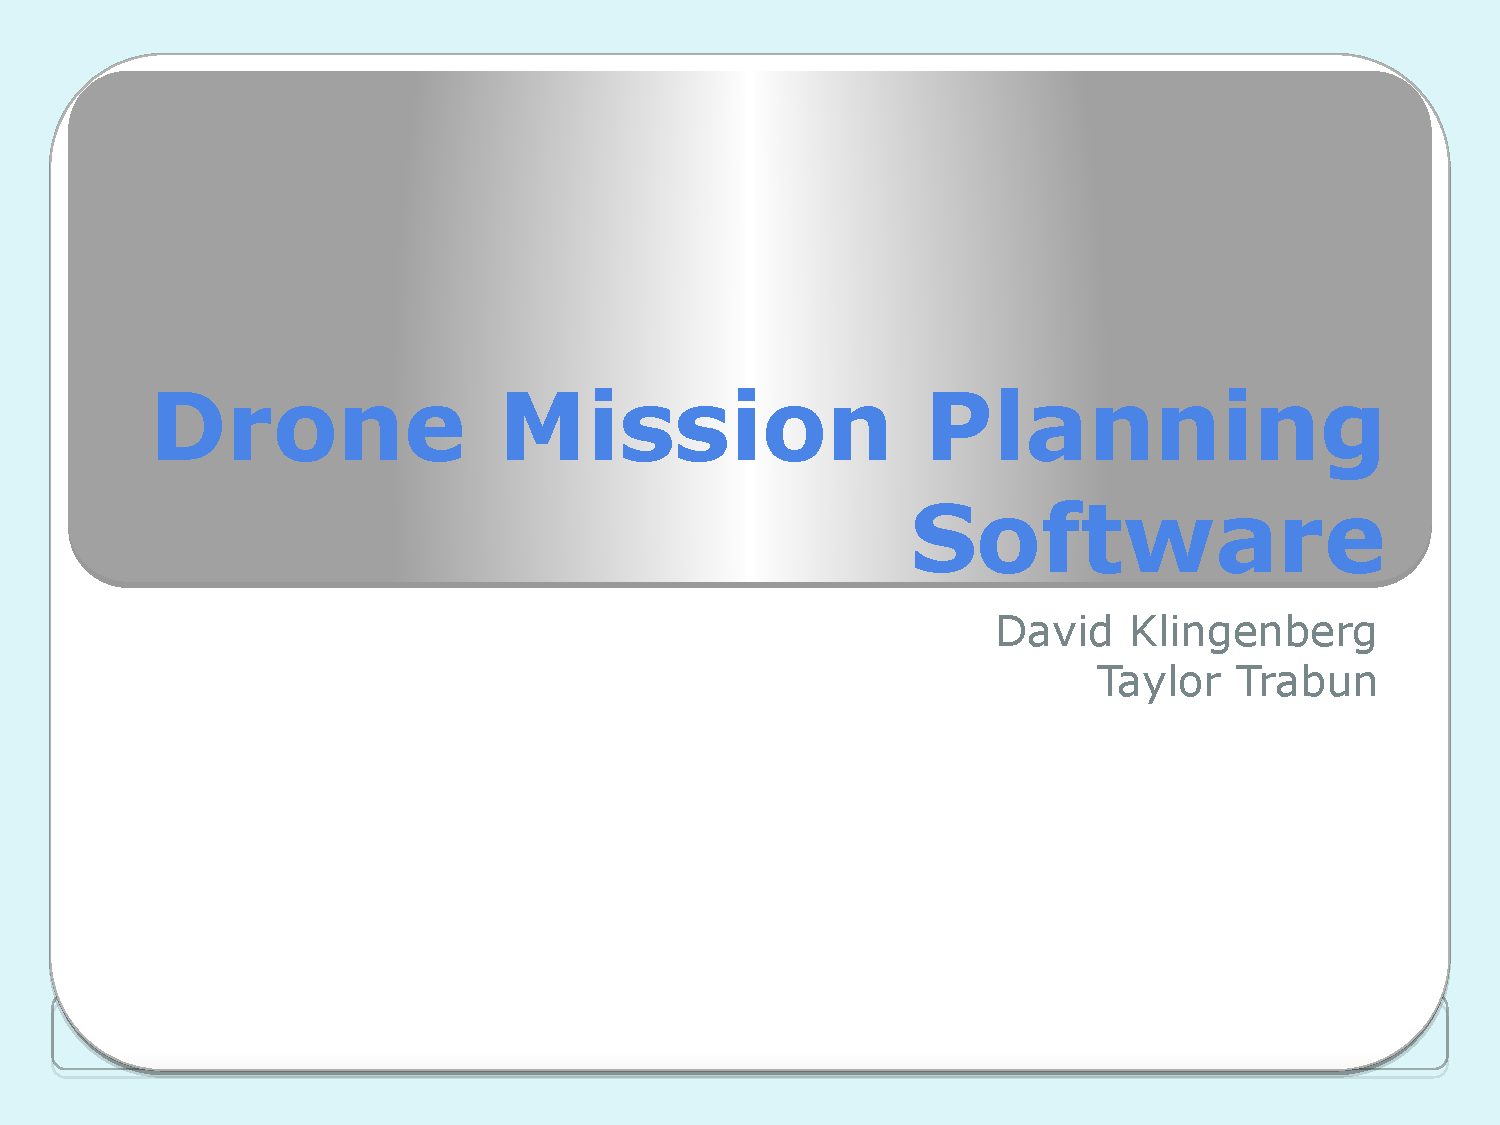
\includepdf[pages={1-9},pagecommand={},width=\textwidth]{./additionalPDF/designReview_revised.pdf}


% Design presentation %%%%%%%%%%%%%%%%%%%%%%%%%%%%%%%%%%%%%%%%%%%%%%%%%%%%%%%%%%%%%%

% Design Doc  %%%%%%%%%%%%%%%%%%%%%%%%%%%%%%%%%%%%%%%%%%%%%%%%%%%%%%%%%%%%%%%%%%%%%%


\documentclass[12pt,a4paper]{article}
\usepackage[utf8]{inputenc}
\usepackage{amsmath}
\usepackage{amsfonts}
\usepackage{amssymb}
\usepackage{graphicx}
\usepackage[margin=1.in]{geometry}


\author{Taylor Trabun}
%\date{A long time ago}
\title{Drone Mission Planning Software: Design Document}
\begin{document}
\maketitle

\section{Introduction}
This document provides the general design of the Drone Mission Planning Software by breaking the entire project down into several components. The current components are the physical drone, the communication system, and the graphical user interface for mission planning.

\section{Drone Design}
The drone design's major requirement that needed to be met was to achieve stable and reliable flight. 

By analyzing the drone, it was determined that its center of gravity was not directly centered on the drone, which resulted in drifting during flight. To remedy this issue, a "part holder" was designed to be mounted on the underside of the drone to hold all the motor controls, which moved the center of gravity to the center of the drone. 

\begin{figure}[h!]

  \centering
    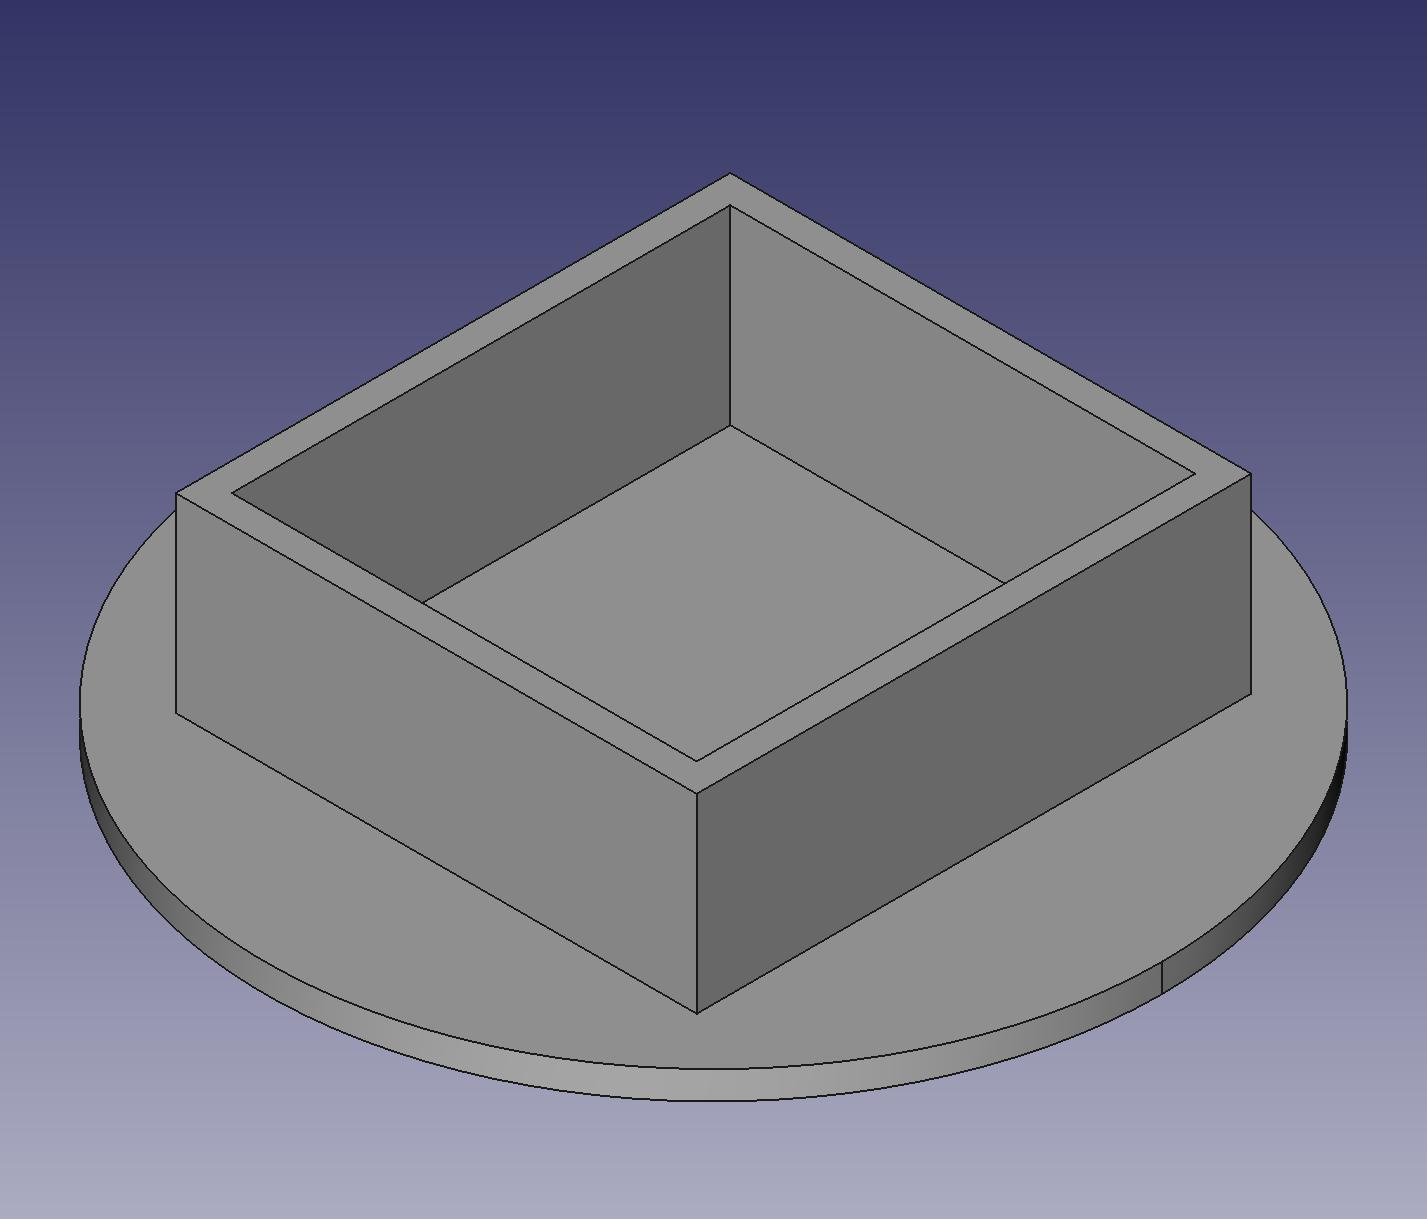
\includegraphics[width=0.45\textwidth]{partbin.jpg}
   \caption{3D sketch of partbin}
\end{figure}


\section{Communication Design}
The communications system needs to follow the following requirements:
\begin{itemize}
	\item Use of XAPI and XBee hardware
	\item Define required TUN packets for communication system 
	\begin{itemize}
		\item Manual drone instructions
		\item Settings and status
		\item ACK
		\item Heartbeat
		\item Override
		\item Flight plan protocol types
	\end{itemize}
\end{itemize}

The following sections will break the communication system down into its several components and detail their design.

	\subsection{Communication Overview}
	Our communications system, as depicted in the graphic below, requires two-way communication between the computer (including the attached Arduino) and the Arduino located on the drone. This system will take an instruction created on the computer, send it over serial to the connected Arduino, pass it to XAPI, XAPI will ship it over XBee to the Arduino on the drone, and a flight control service will execute the instruction. 
	
	\begin{figure}[h!]

  		\centering
    	\includegraphics[width=0.5\textwidth]{droneControlSequence.png}
   		\caption{Overview of communications system}
	\end{figure}
	
	\subsection{Hardware Components}
	Our current communications requires the following hardware components:
	\begin{itemize}
		\item Arduino Mega 2560
		\item XBee modules
		\item LCD Shields (for development and debugging)
		\item Serial add-on for Arduino
		\item A computer running Windows to communicate with base Arduino (Workstation needs to be able to run C\# programs)
	\end{itemize}
	
	\subsection{XAPI}
	To satisfy one of our major requirements, we run the XAPI on each Arduino in the communications system. 
	
	XAPI is, put simply, a micro-controller service manager that communicates, both internally and externally, using TUN packets. When communicating externally, the XAPI ships the TUN packet using the XBee hardware by embedding the TUN packet in a XBee packet.
	
	Each service available with the API use XAPI to communicate, using XAPI as the core that each service "latches" to. For instance, if a chat service wanted to display a message on a attached LCD screen, the following steps would be carried out:
	\begin{enumerate}
		\item Chat service creates a LOCAL\_ LCD TUN packet
		\item Chat service passes the newly created packet to the XAPI core
		\item XAPI places the packet in its internal packet buffer
		\item The LCD service latch queries XAPI for any packets designated for the LCD service
		\item LCD service grabs LOCAL\_ LCD TUN packet
		\item LCD service processes and displays the packet
	\end{enumerate}
	
To satisfy our project's requirements, we need to design a Flight Control service that will be able to handle any instruction packets and translate them to instructions that can be given to the drone's flight computer. In addition to this, there is a requirement for a Mission Plan service that will store and execute flight plan's designed by the user and sent to the drone.
	
\section{Graphical User Interface Design}
The graphical user interface must satisfy several requirements:
\begin{enumerate}
	\item Must be user-friendly
	\item Allow 3-dimensional mission planning
	\item Allow upload of flight plan to drone
	\item Allow manual override
\end{enumerate}

Given these requirements we were able to design a general design for the graphical user interface (GUI), as shown below. This GUI is split into several sections that convey different information, that in some cases can be adjusted. 

We have a flight control section (light-blue) that shows the status of the drone components and allows the user to "zero out" each component or take manual control. The status information section (yellow) shows different readings from the drone's on-board instruments. The flight planning system (light-red) will be where the user can develop a flight plan to be uploaded to the drone (note that this functionality is still under design and may end up being a separate window that needs to be opened up). The final section is the communications terminal (light-green) that displays all packets sent and received on the Arduino attached to the source computer. This communications terminal will allow the user to see that the drone is still connected and will allow for easy communications debugging.

	\begin{figure}[h!]

  		\centering
    	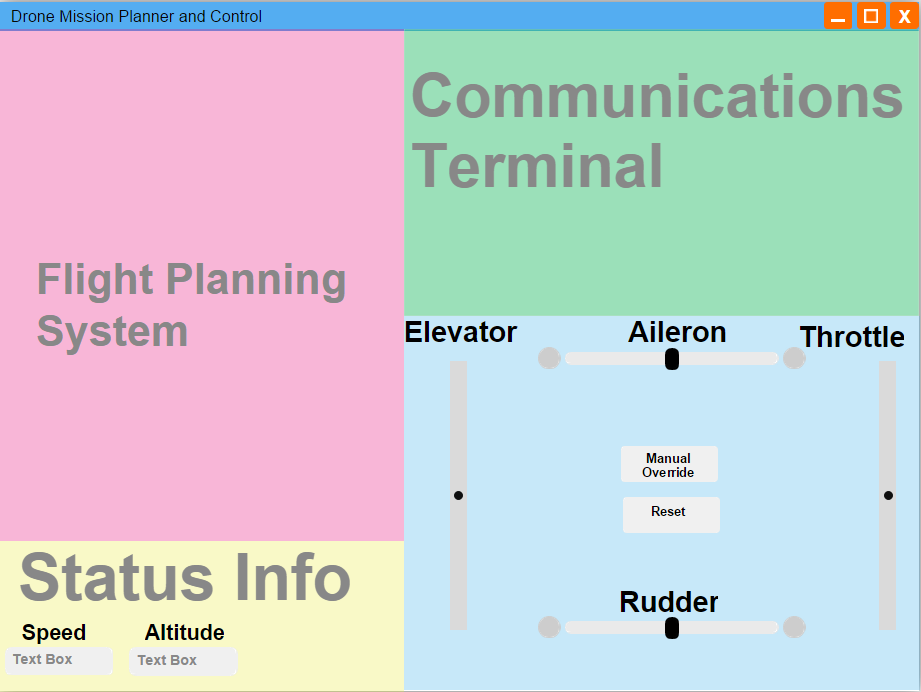
\includegraphics[width=0.75\textwidth]{guiMockup.png}
   		\caption{Graphical user interface mock-up design}
	\end{figure}


\end{document}

% Design Doc  %%%%%%%%%%%%%%%%%%%%%%%%%%%%%%%%%%%%%%%%%%%%%%%%%%%%%%%%%%%%%%%%%%%%%%

\clearpage
\appendix
\appendixpage	
\addappheadtotoc

\section{Miscellaneous UML Charts}
\label{sec:appUML}
\begin{figure}[!h]
	\centering
		\includegraphics[width=0.5\textwidth]{./plantUML/droneControlSequence.png}
	\caption{Communication Sequence}
	\label{fig:comseq}
\end{figure}

\begin{figure}[!h]
	\centering
		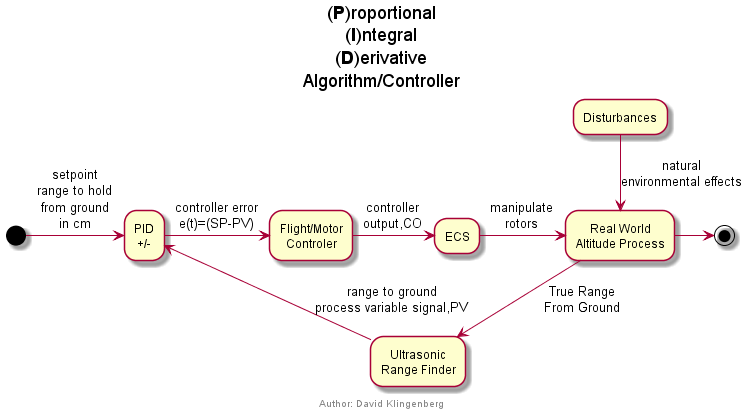
\includegraphics[width=0.5\textwidth]{./plantUML/PIDloop}
	\caption{PID Controller}
	\label{fig:PIDloop}
\end{figure}

\clearpage
\section{ATMEL\textsuperscript{\textcopyright} Microcontrollers}
\label{sec:appATMEL}
\begin{figure}[!h]
	\centering
		\includegraphics[width=.8\textwidth]{./additionalPDF/Atmel-644.pdf}
	\caption{ATmega644}
	\label{fig:ATmega644}
\end{figure}

\begin{figure}[!h]
	\centering
		\includegraphics[width=.8\textwidth]{./additionalPDF/Atmel-2560.pdf}
	\caption{ATmega2560}
	\label{fig:ATmega2560}
\end{figure}

\clearpage

\section{Technical Drawings}
\label{sec:TechDraw}

\begin{figure}[!h]
	\centering
		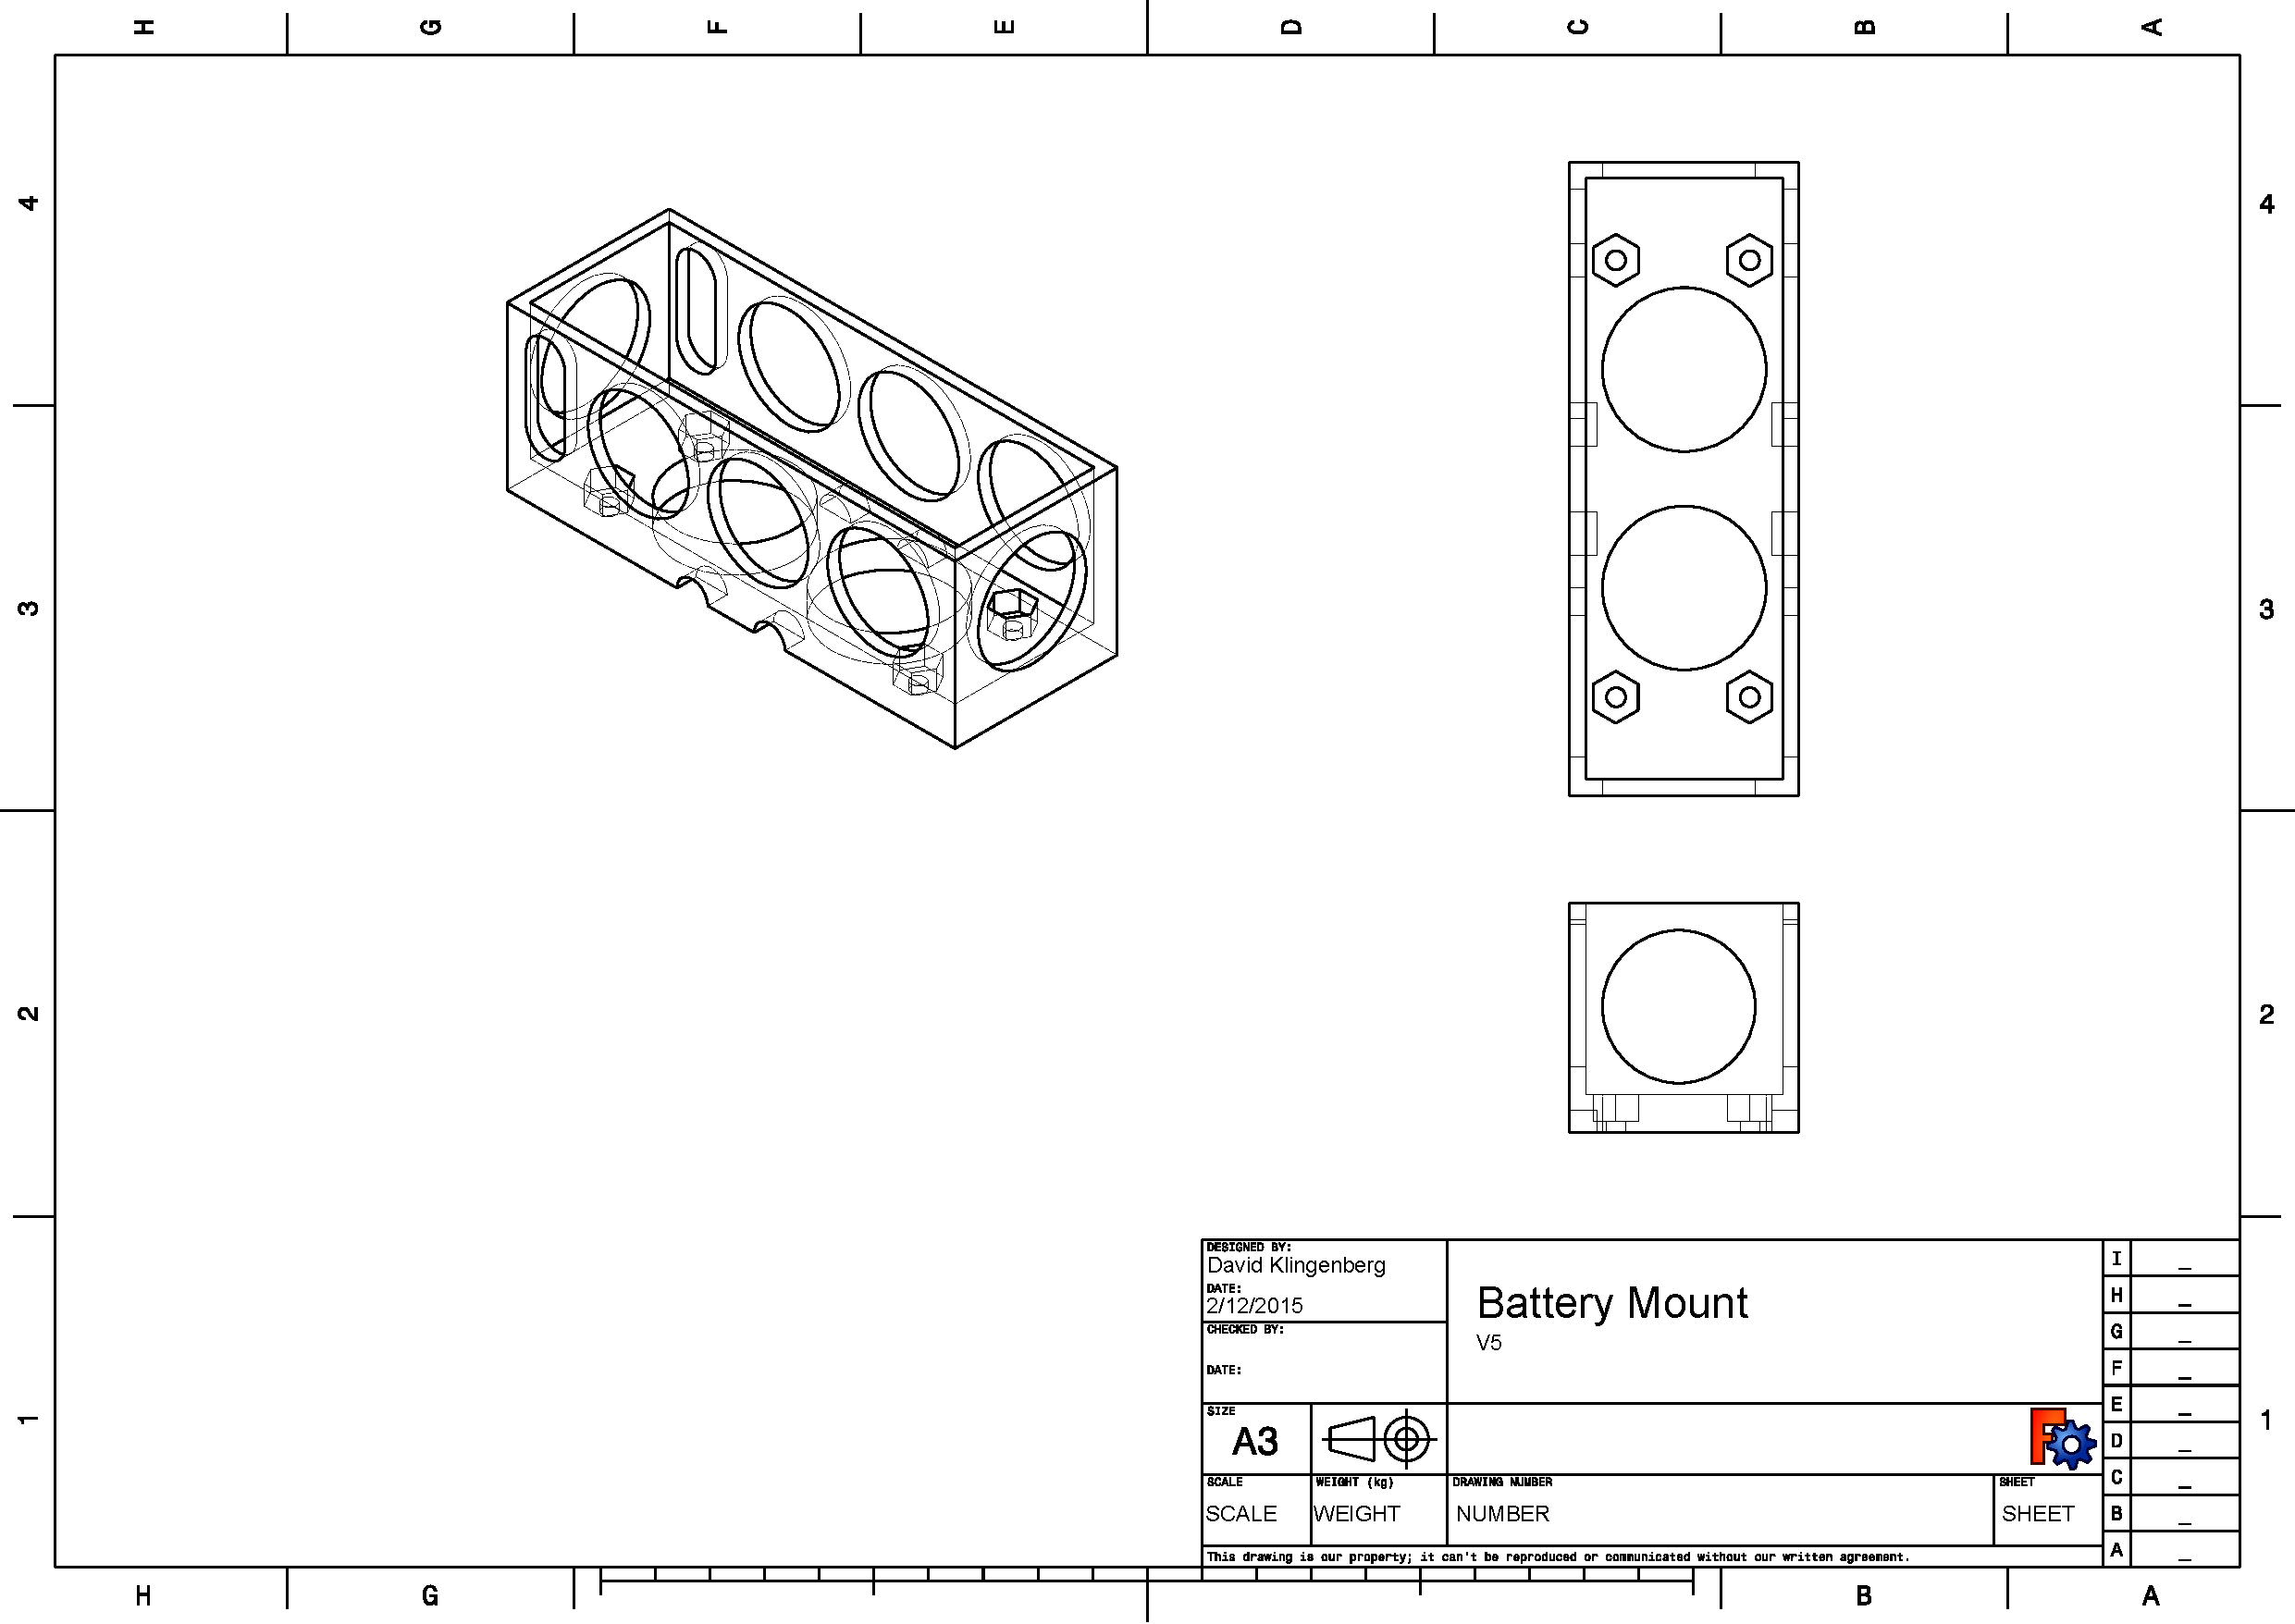
\includegraphics[width=1\textwidth]{./graphics/BatteryBoxV5-eps-converted-to.pdf}
	\caption{Battery Bracket}
	\label{fig:BattBin}
\end{figure}

\begin{figure}[!h]
	\centering
		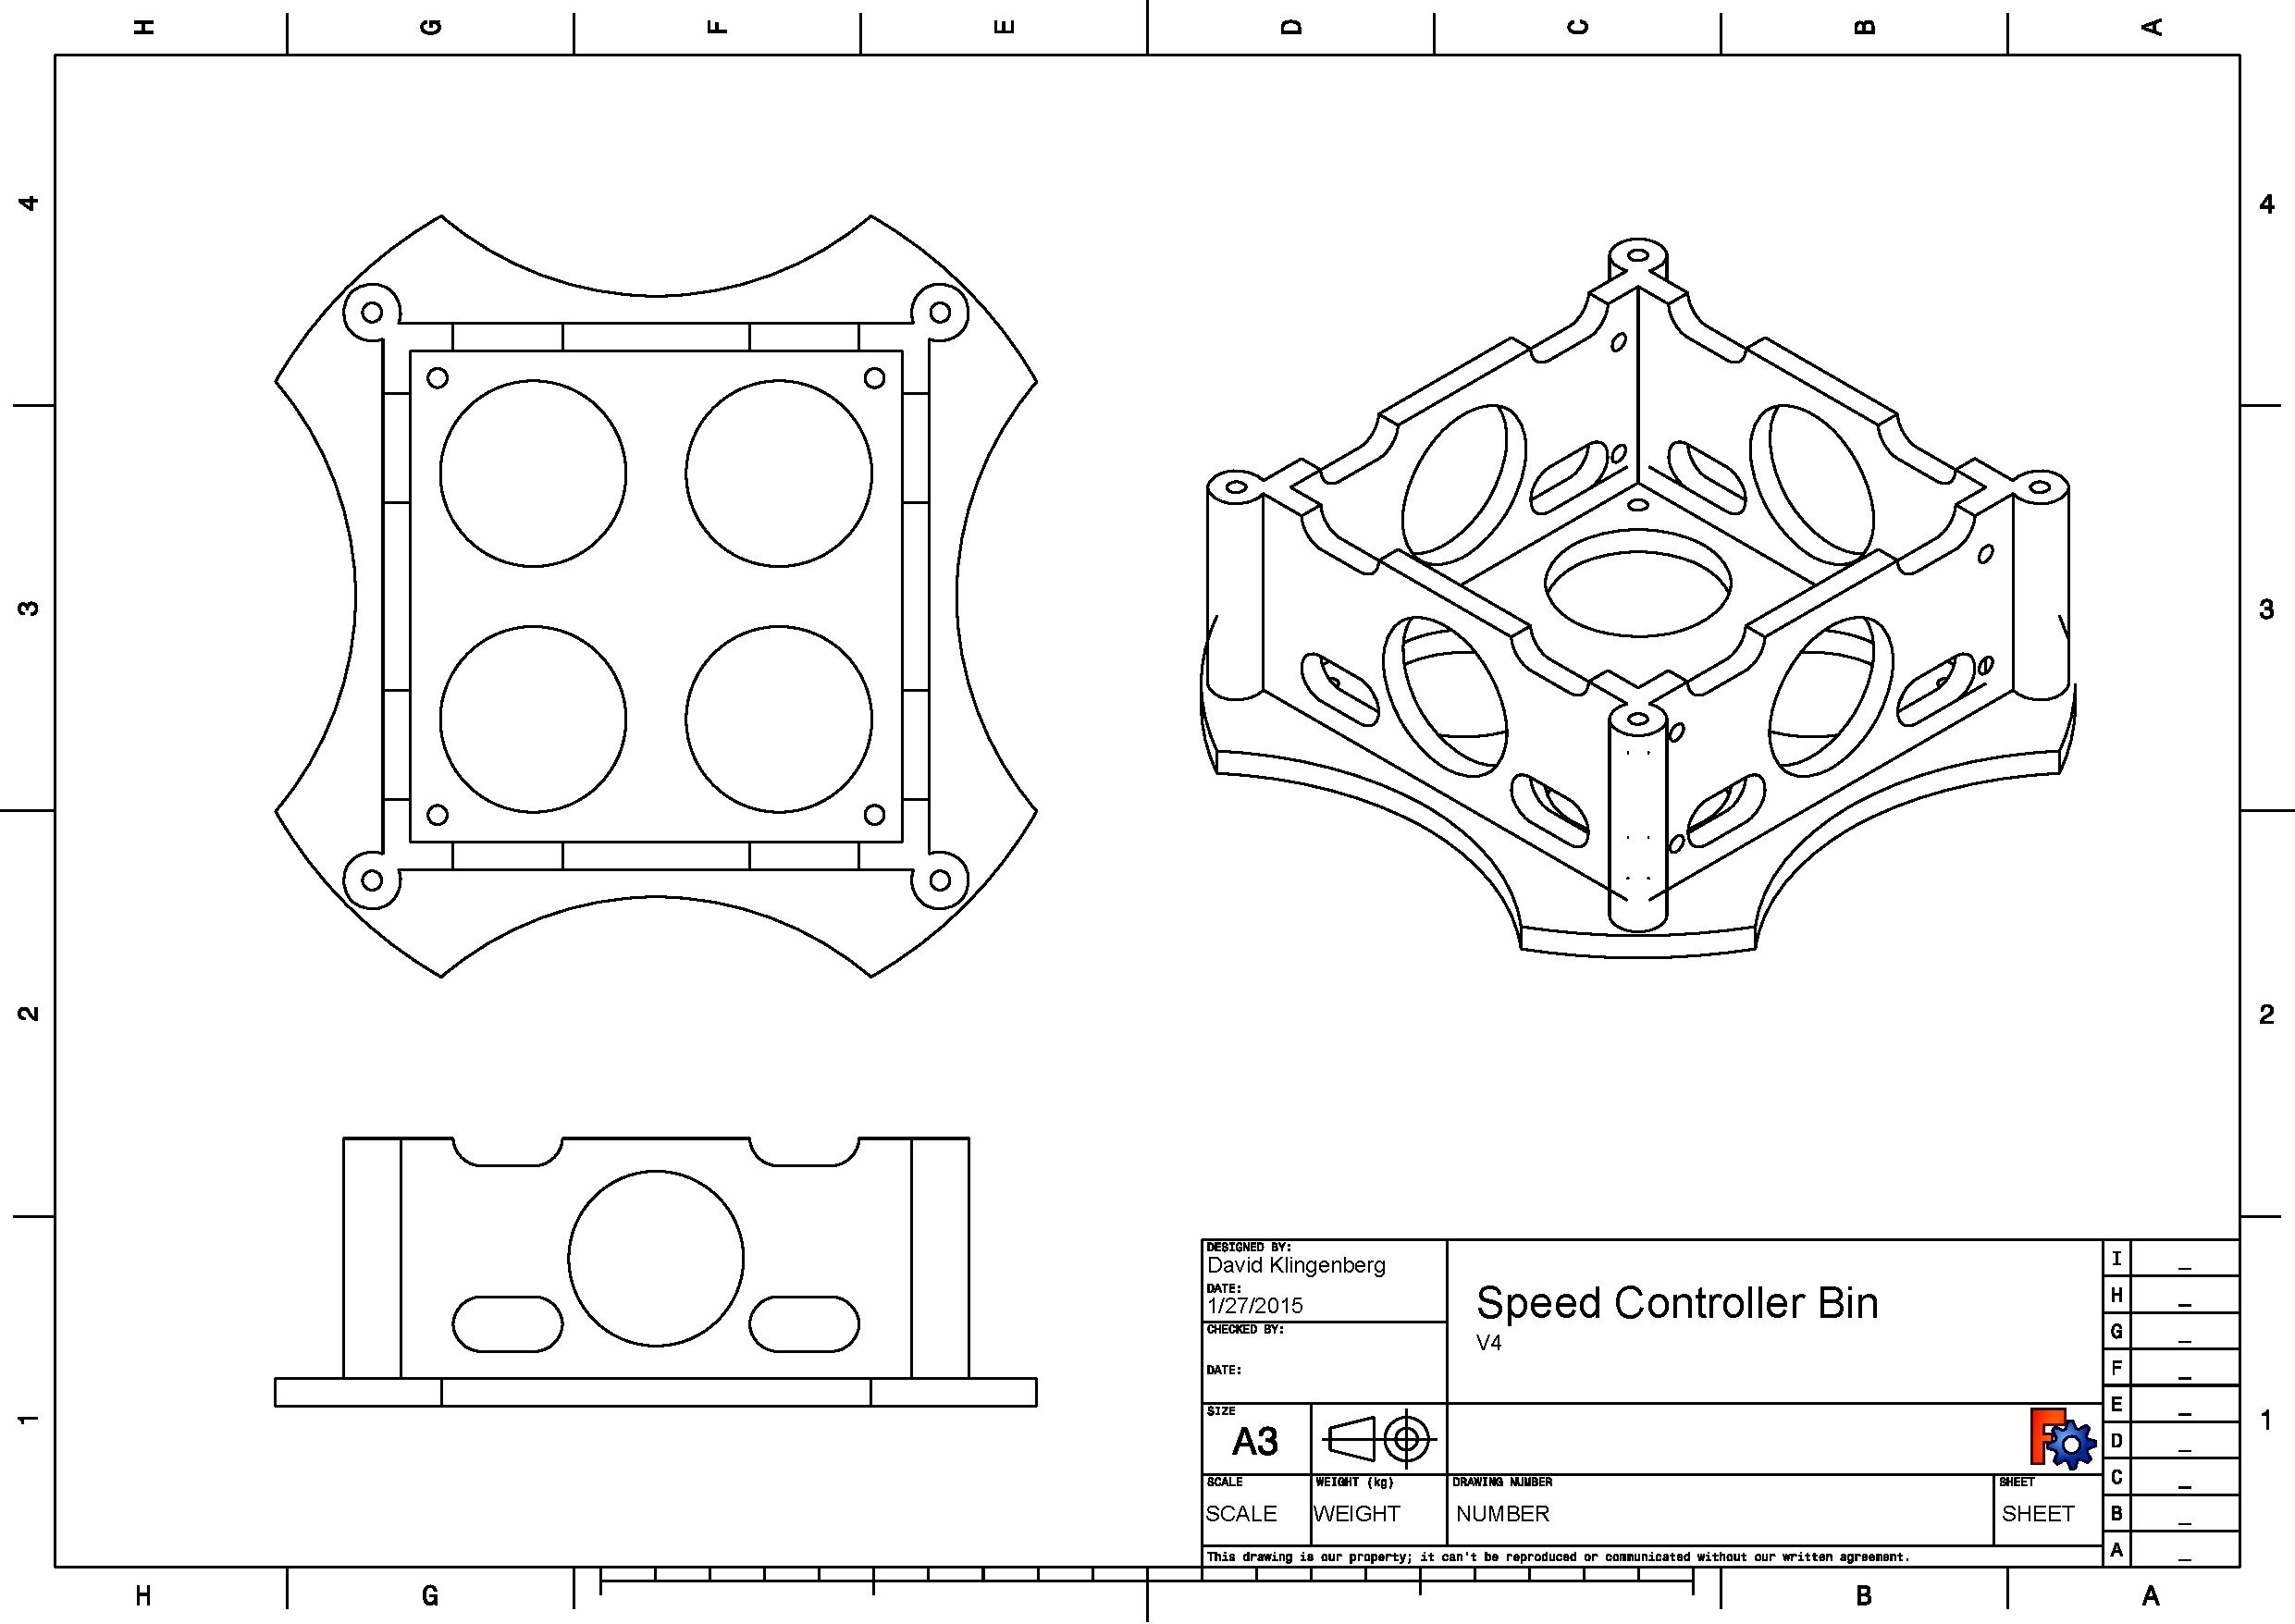
\includegraphics[width=1\textwidth]{./graphics/Speed_controler_bin-eps-converted-to.pdf}
	\caption{Electronic Speed Controller Bracket}
	\label{fig:partbin}
\end{figure}

\begin{figure}[!h]
	\centering
		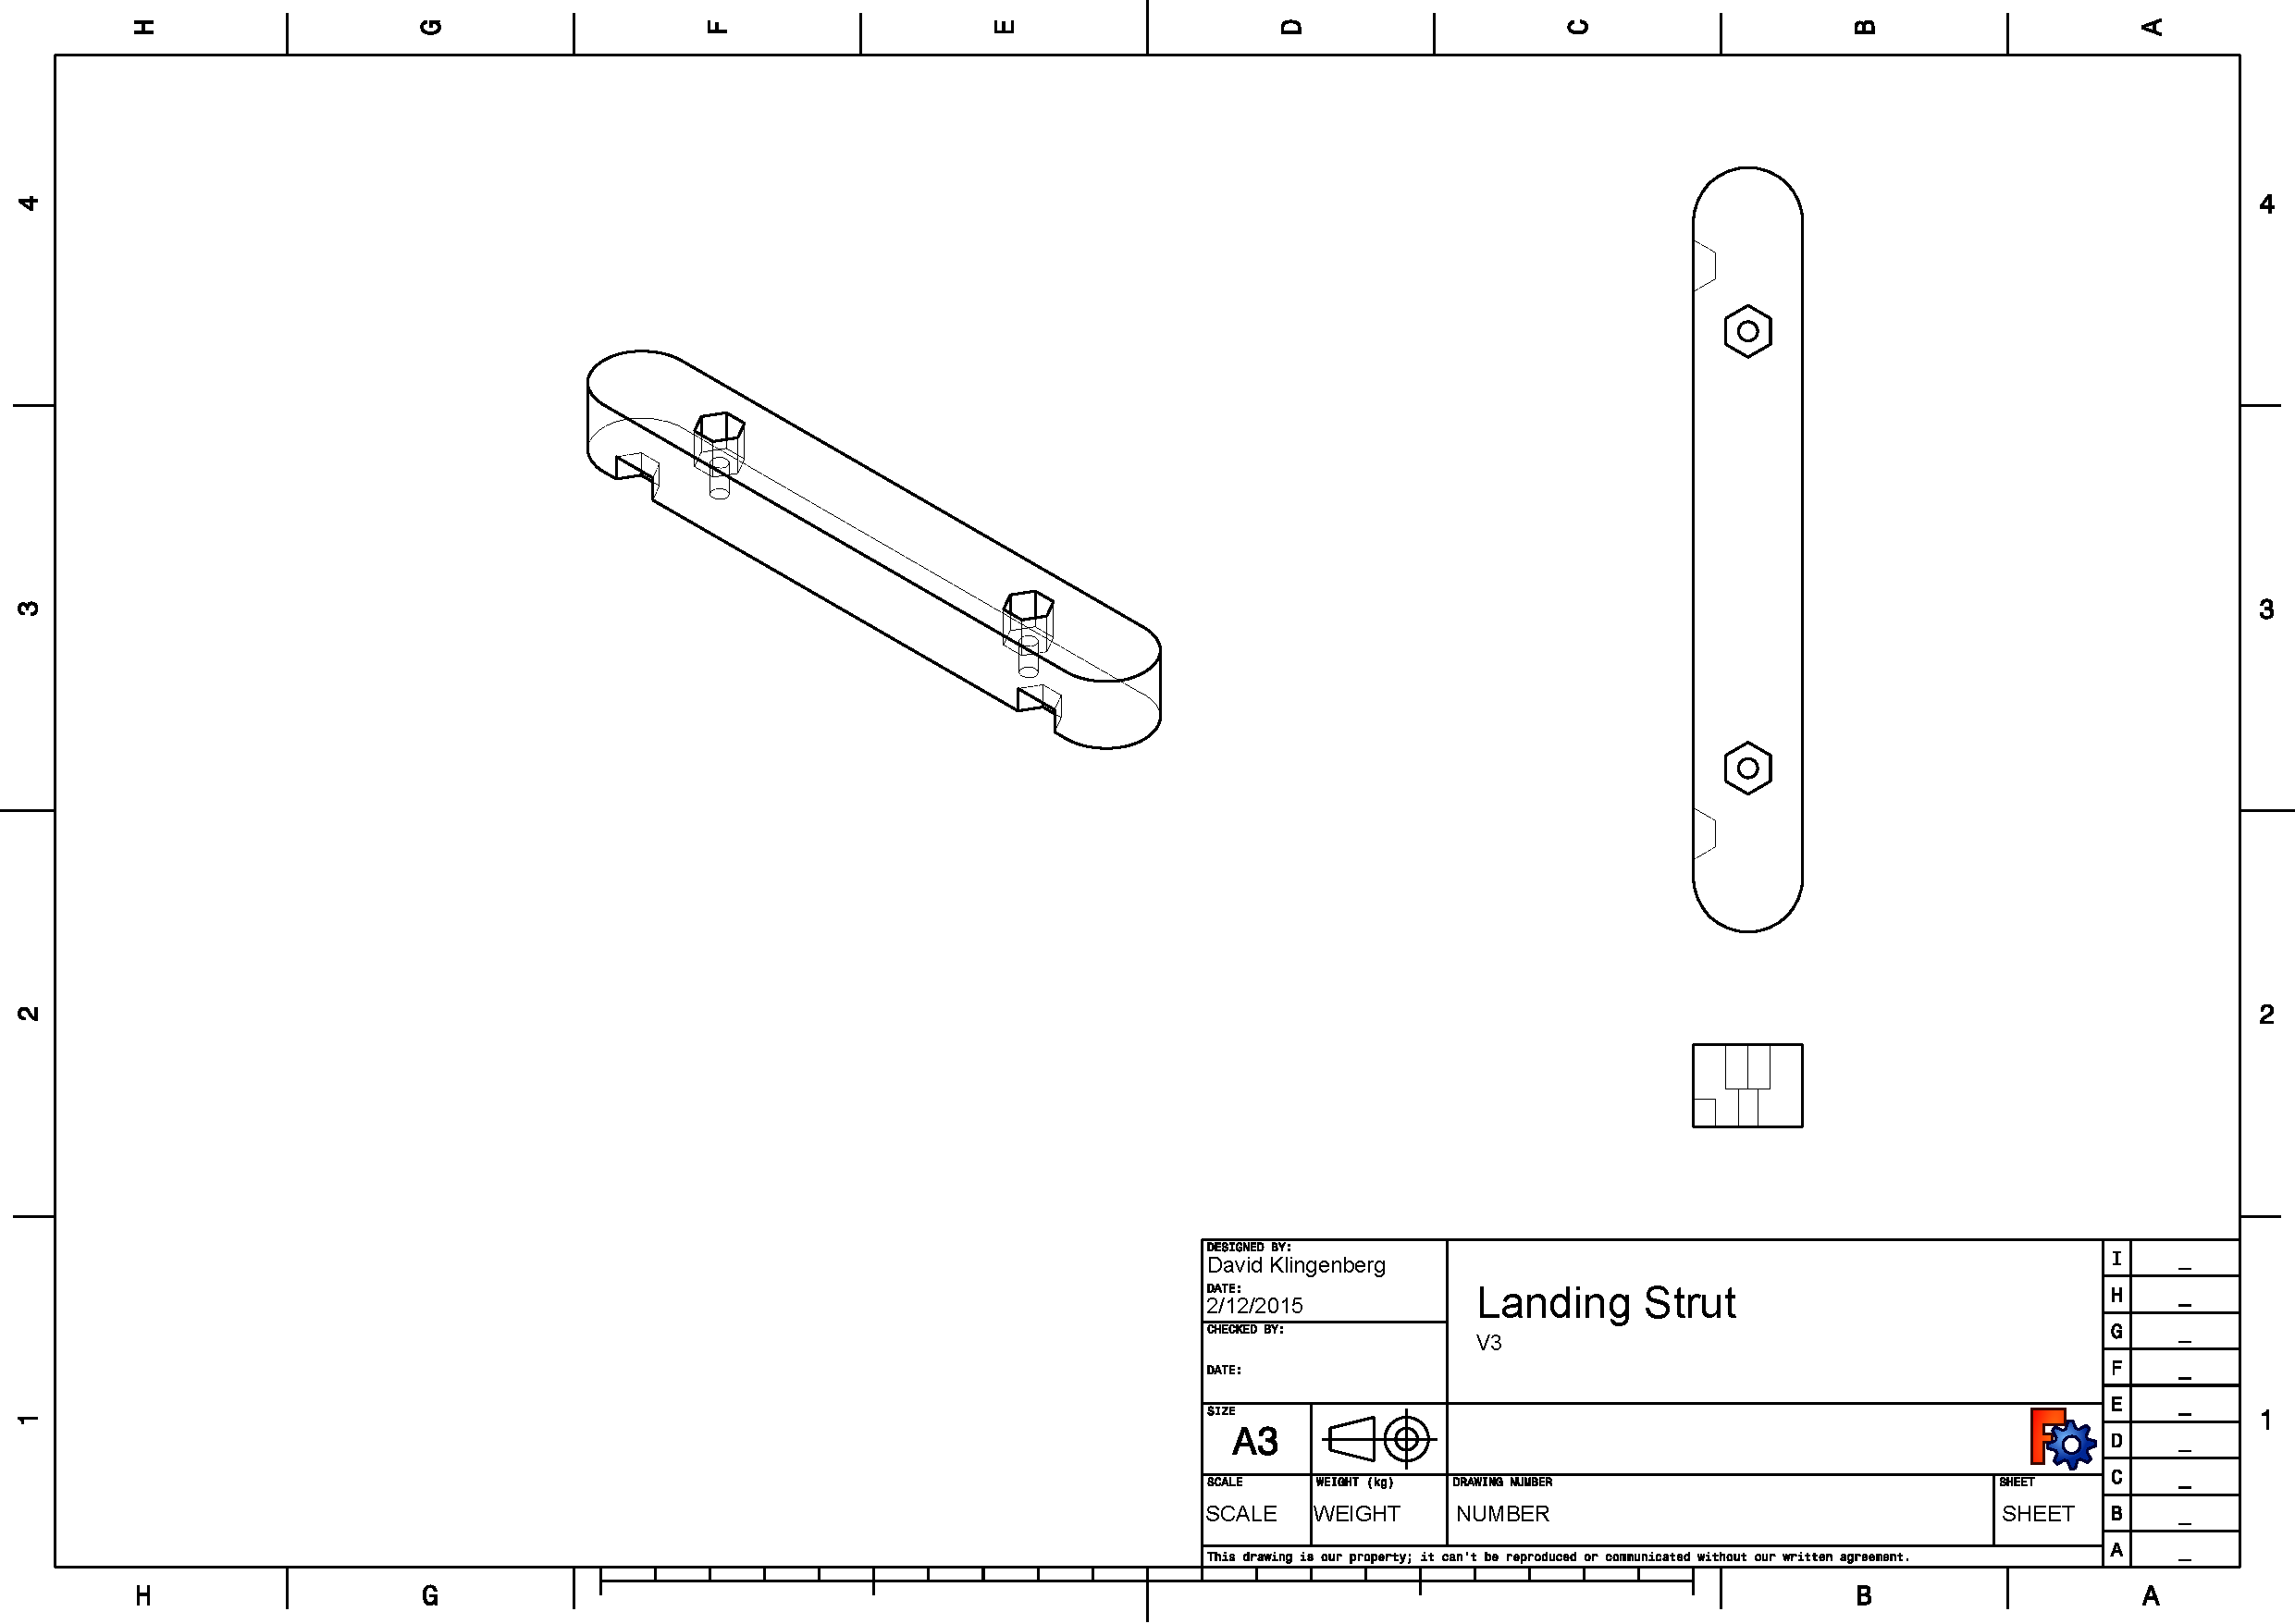
\includegraphics[width=1\textwidth]{./graphics/Landing_strut-eps-converted-to.pdf}
	\caption{Landing Strut}
	\label{fig:landingStrut}
\end{figure}

\begin{figure}[!h]
	\centering
		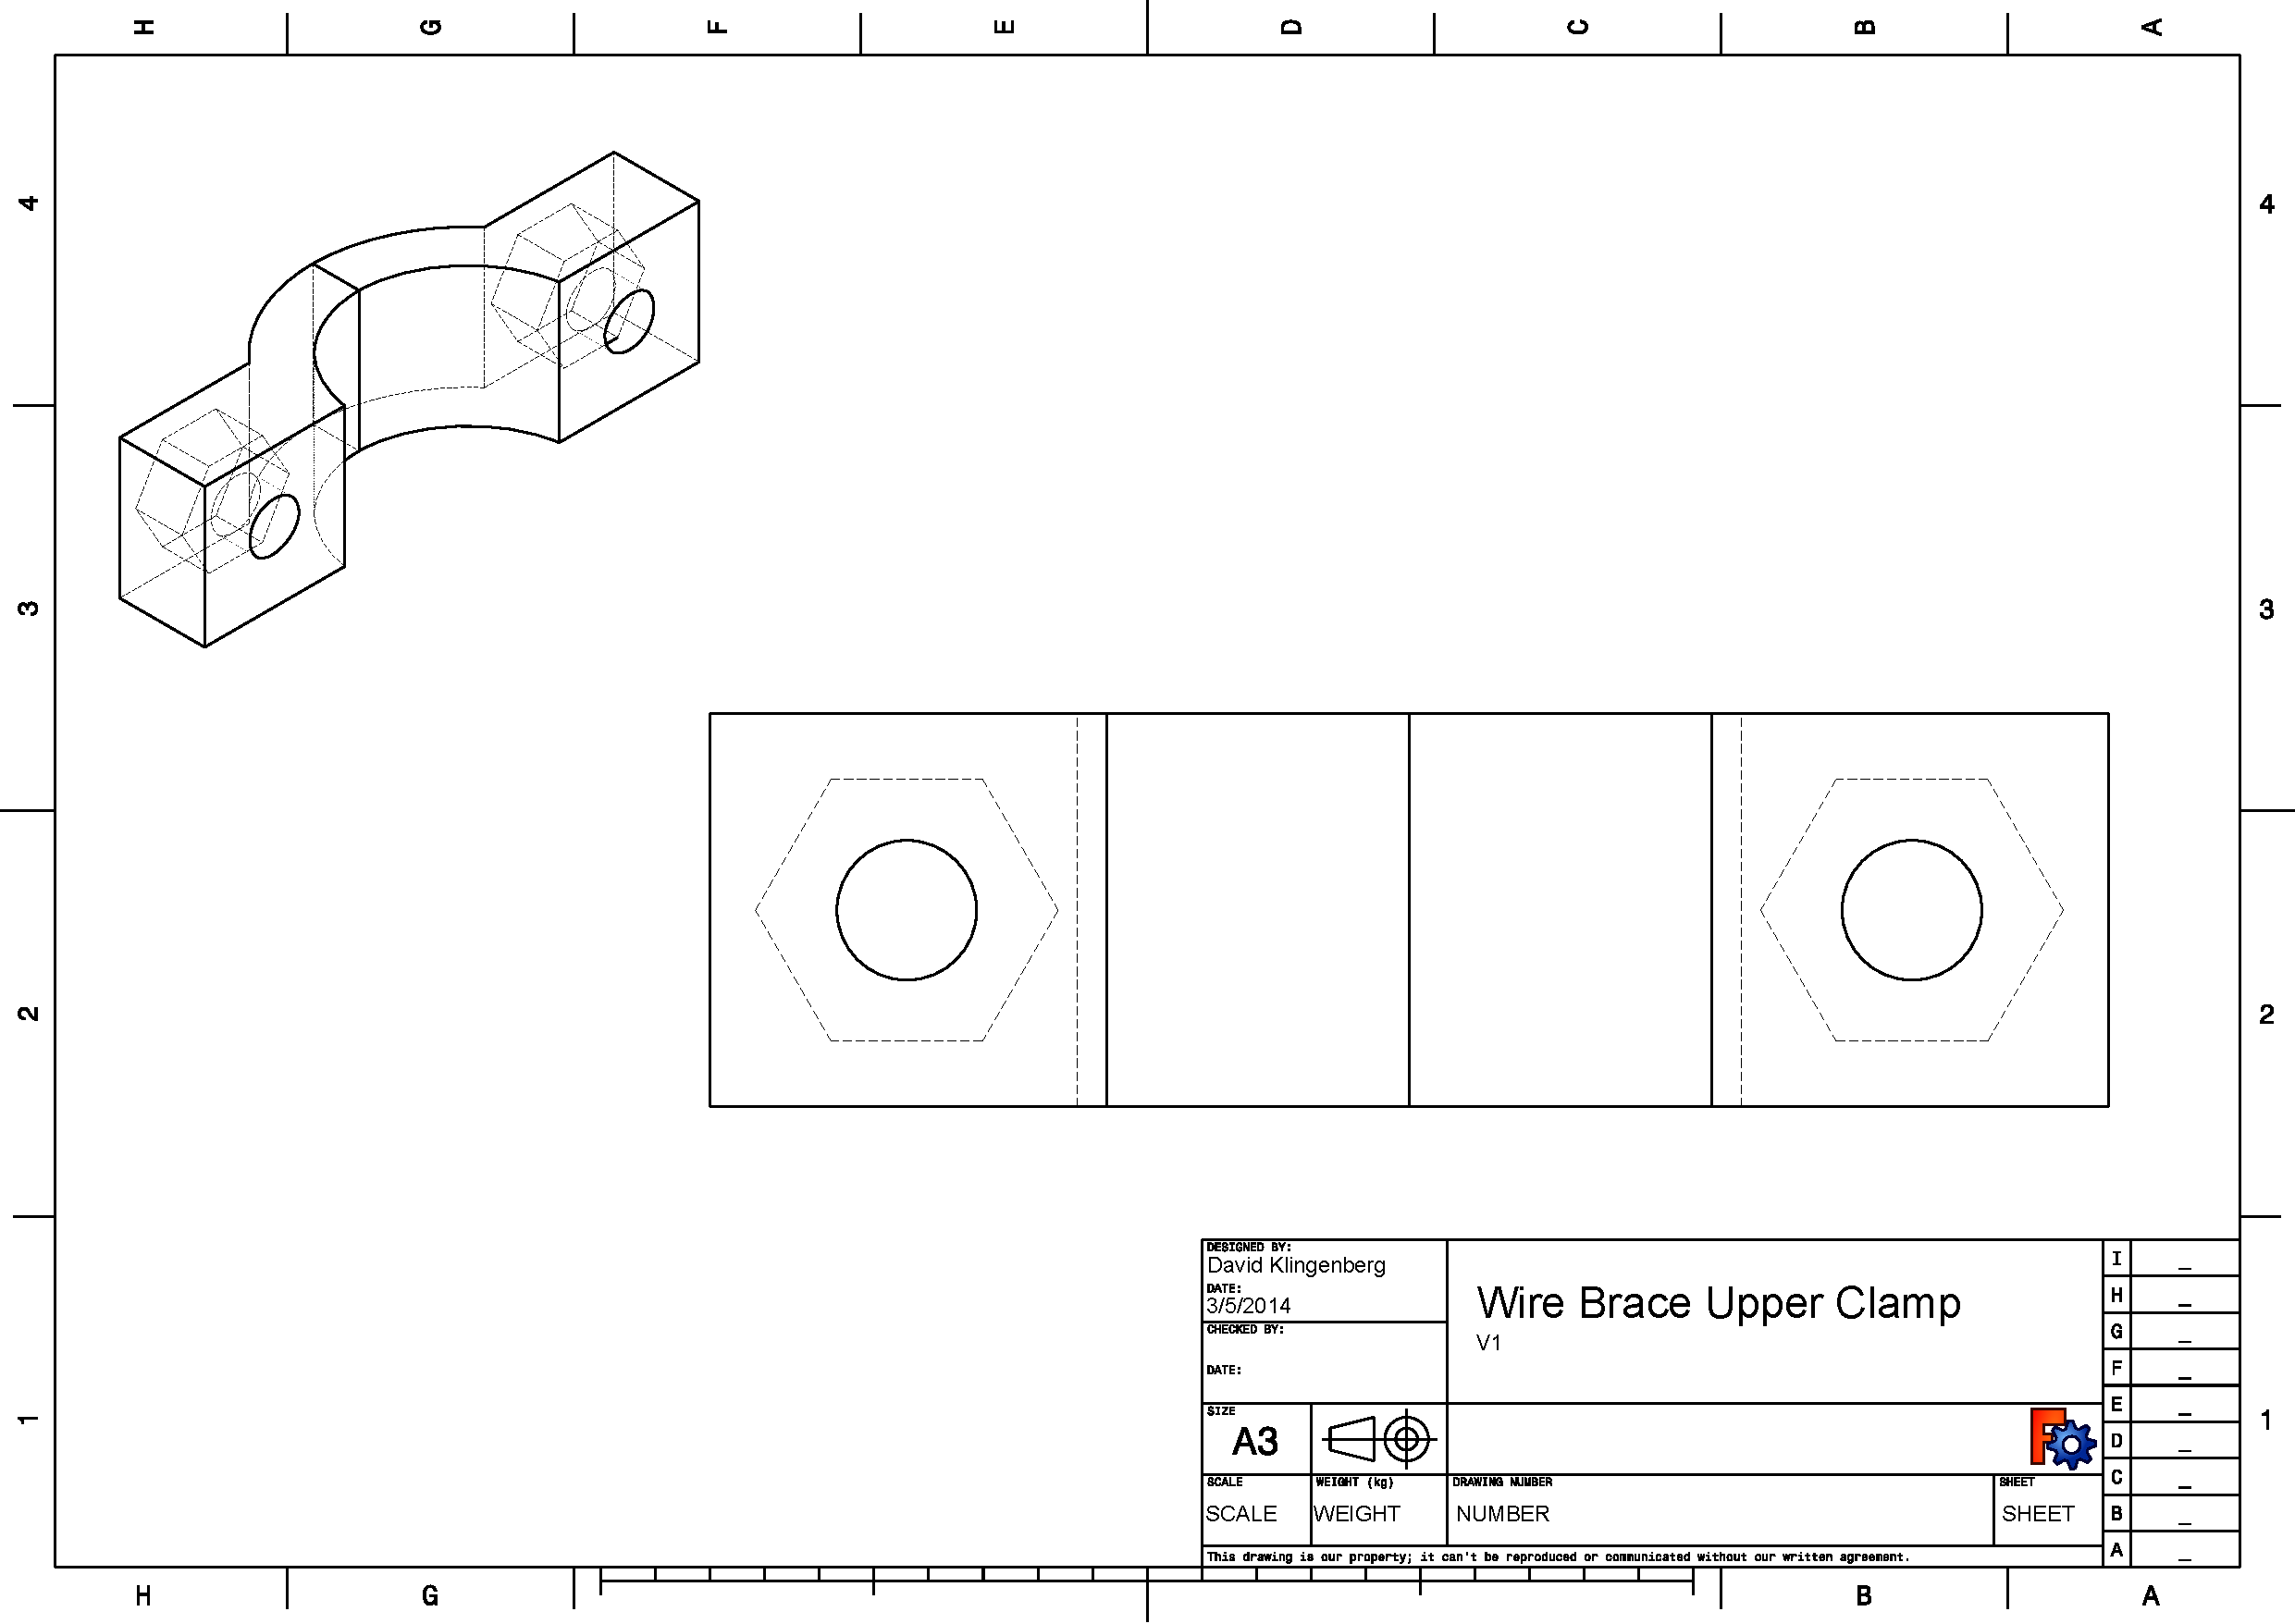
\includegraphics[width=1\textwidth]{./graphics/wire_brace_uper_clamp-eps-converted-to.pdf}
	\caption{Wire Brace Upper Clamp}
	\label{fig:wirebraceupperclamp}
\end{figure}


\begin{figure}[!h]
	\centering
		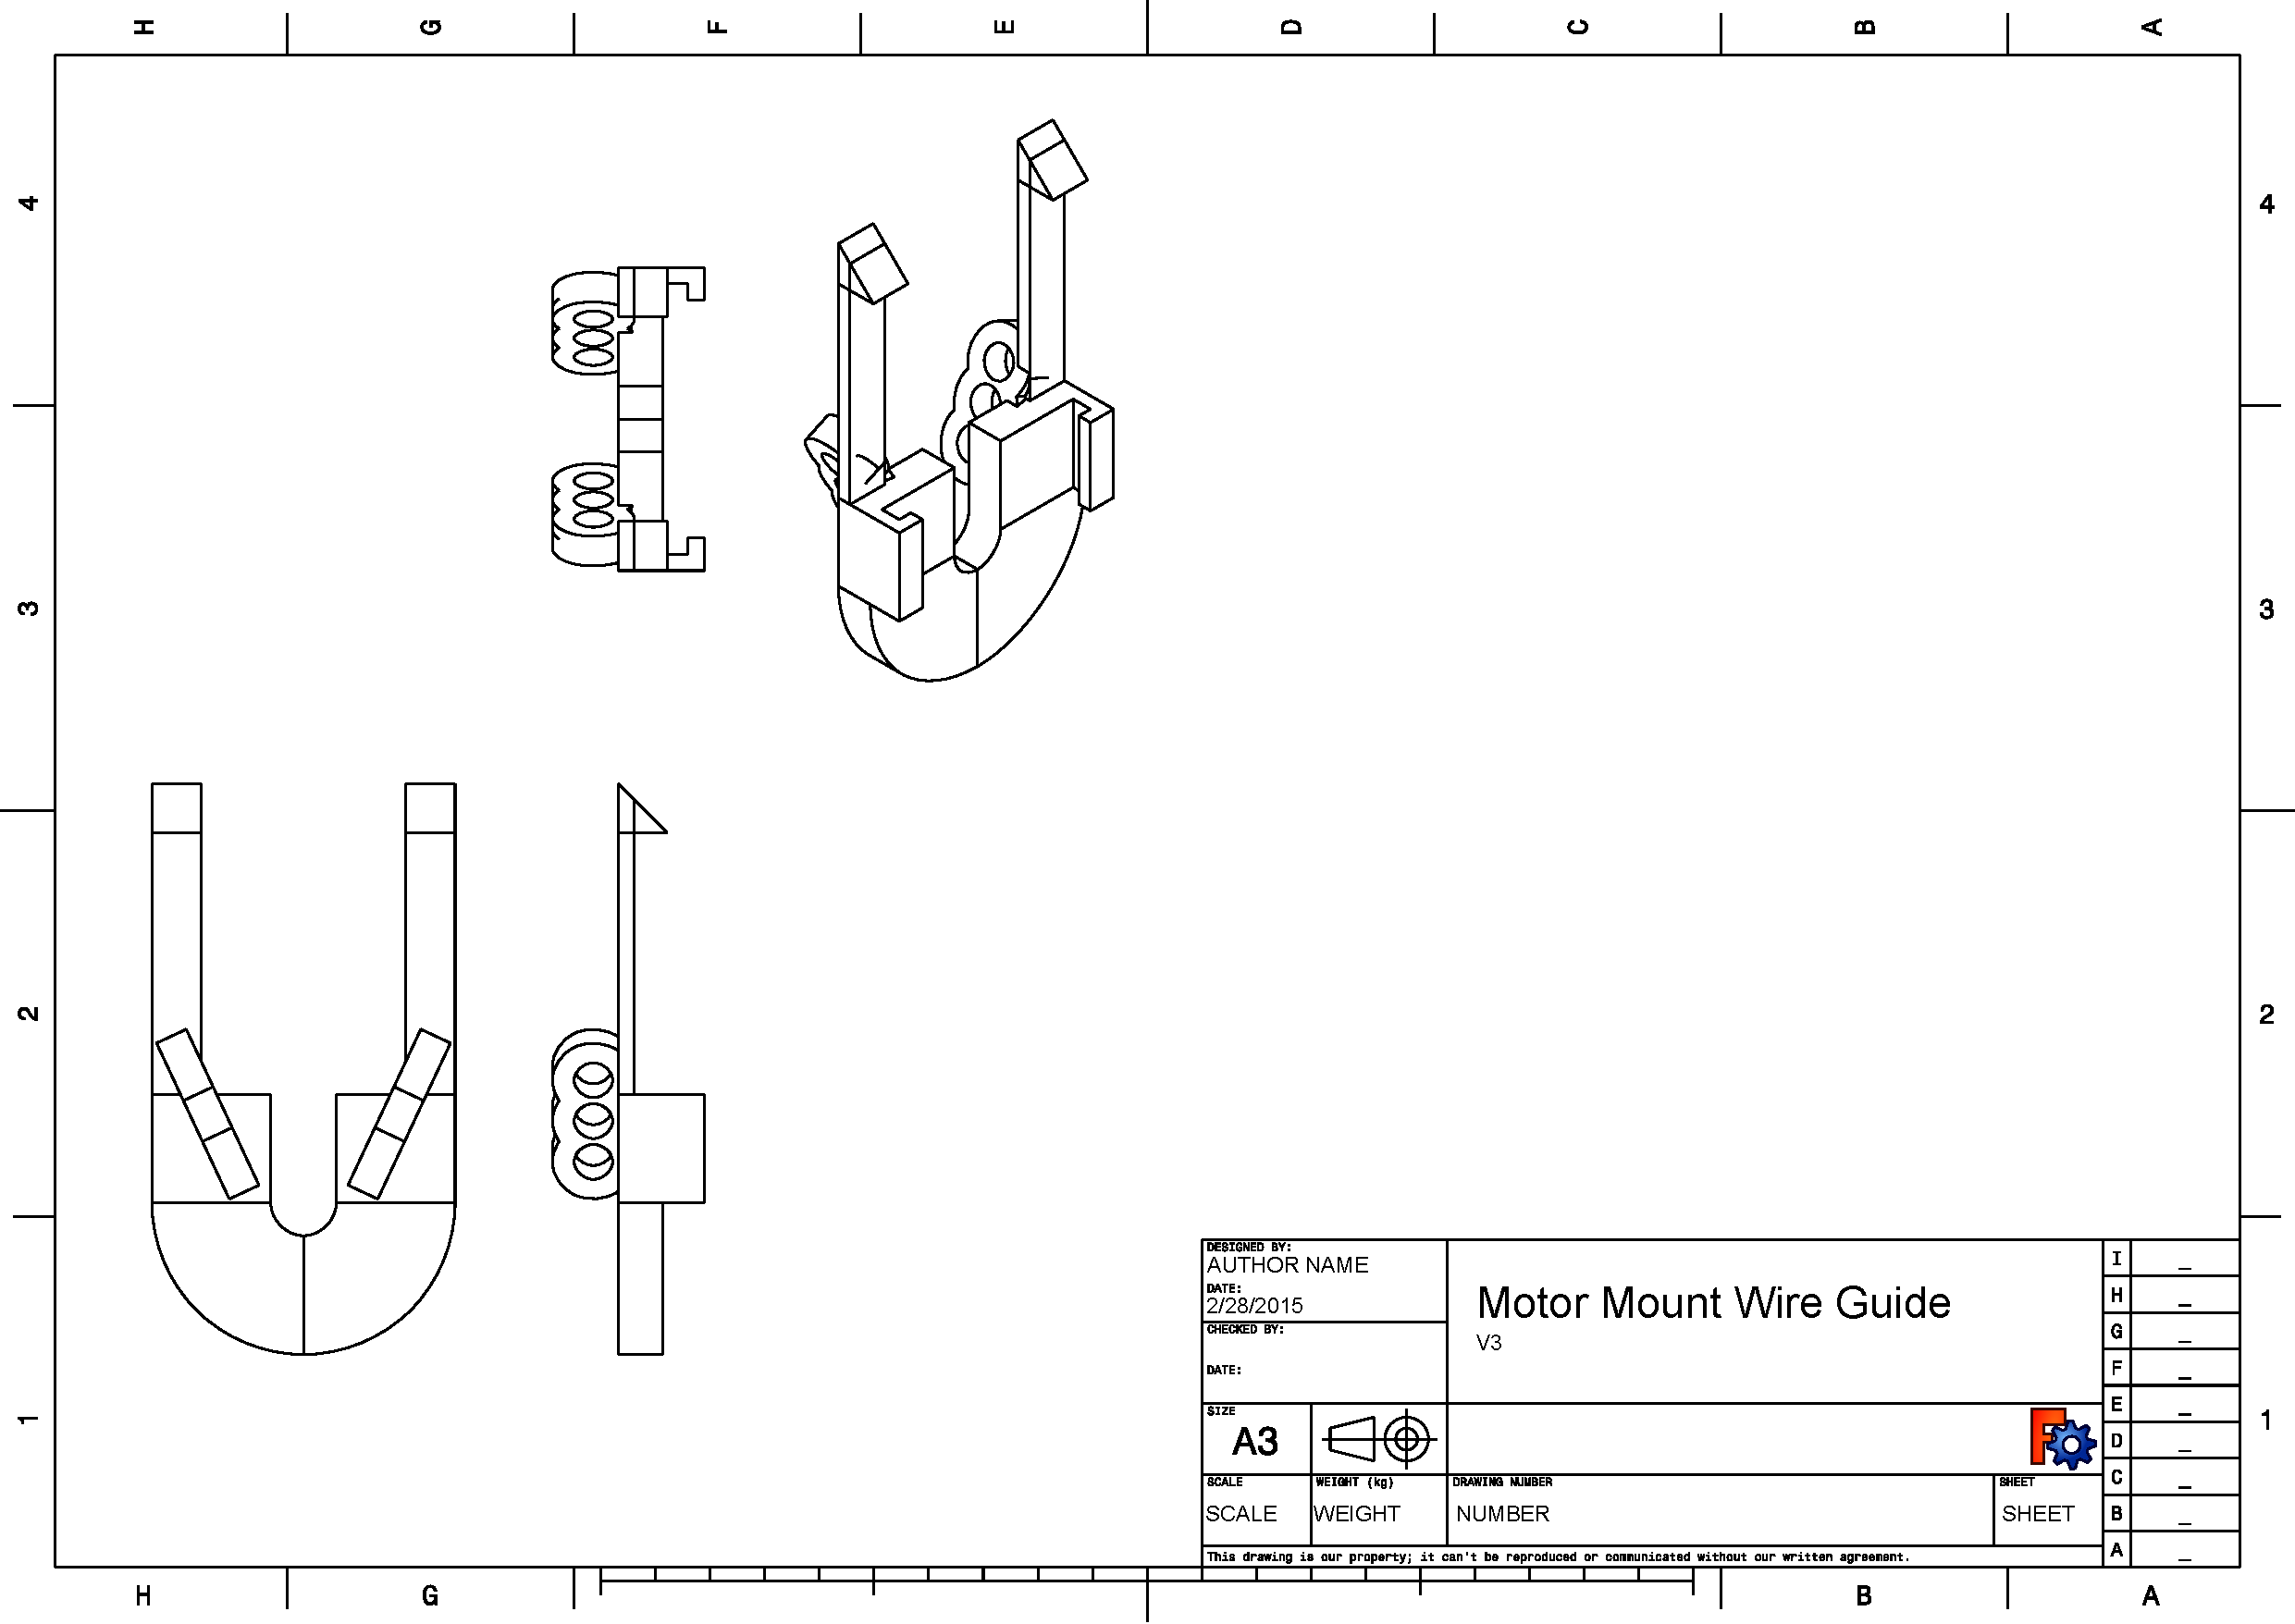
\includegraphics[width=1\textwidth]{./graphics/MotorMountWireBracket-eps-converted-to.pdf}
	\caption{Motor Mount Wire Brace}
	\label{fig:motormountwirebrace}
\end{figure}

\begin{figure}[!h]
	\centering
		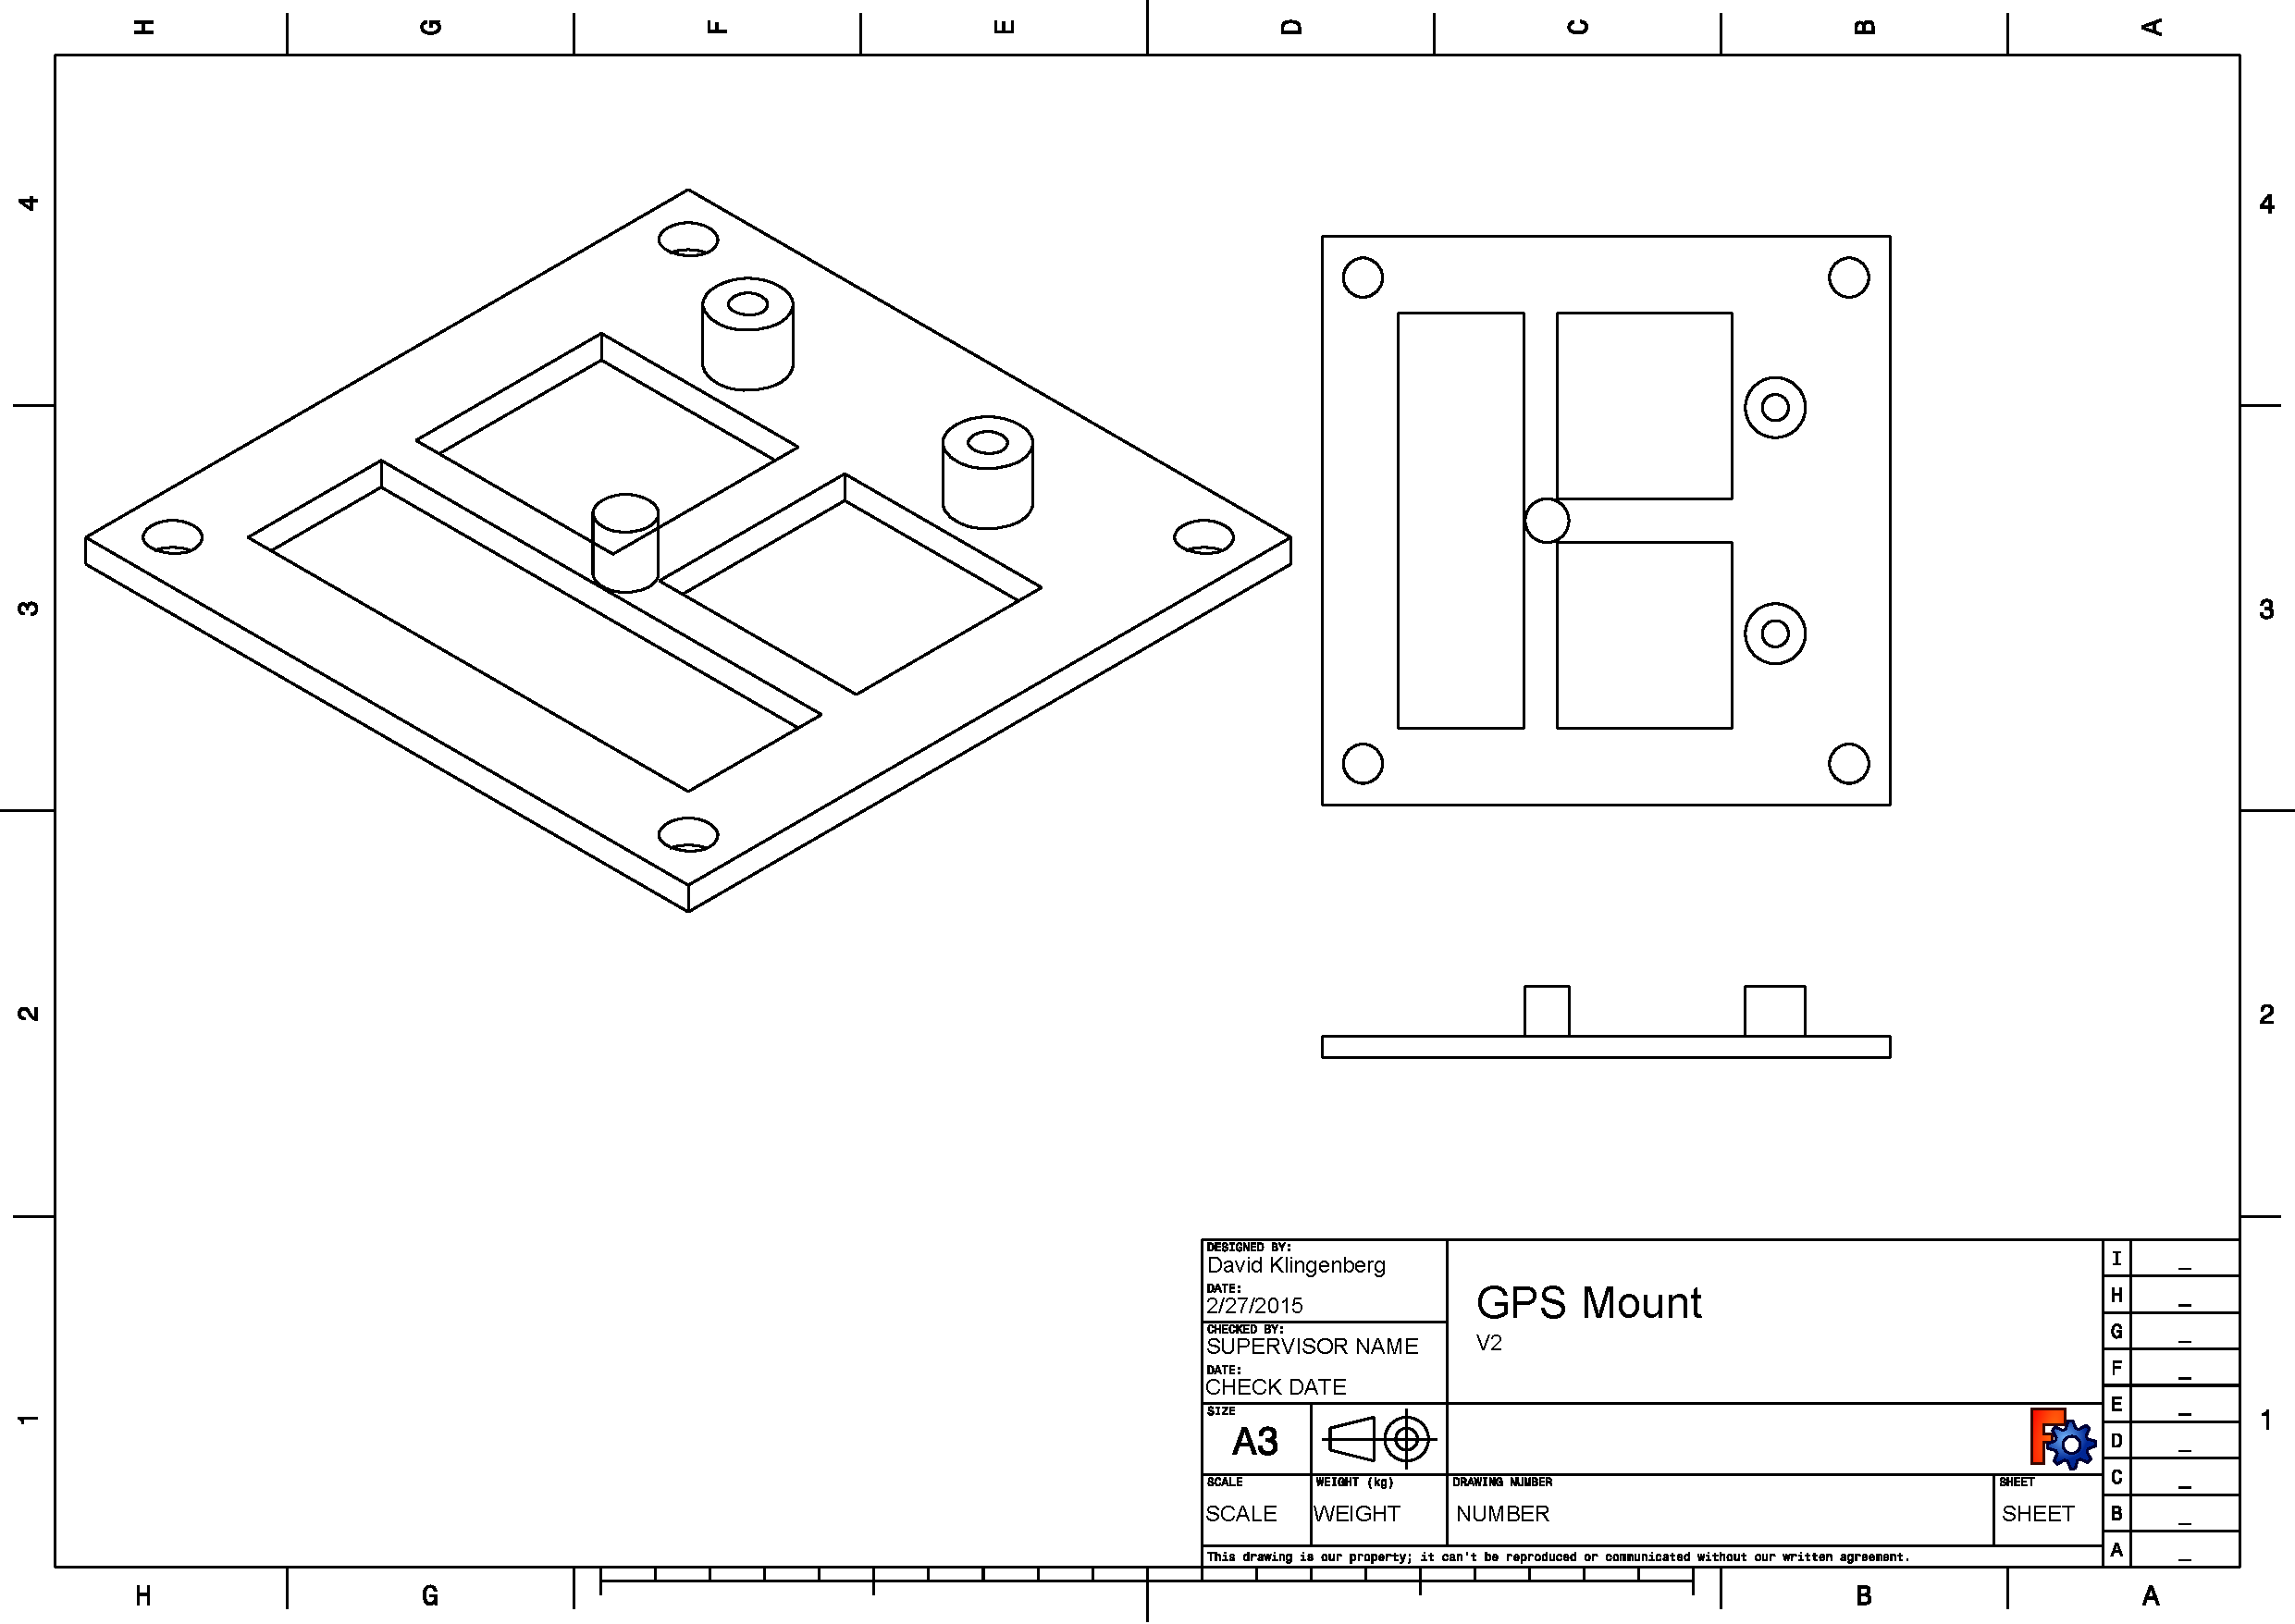
\includegraphics[width=1\textwidth]{./graphics/gps_mountV2-eps-converted-to.pdf}
	\caption{Gps Mount}
	\label{fig:gpsmount}
\end{figure}

\begin{figure}[!h]
	\centering
		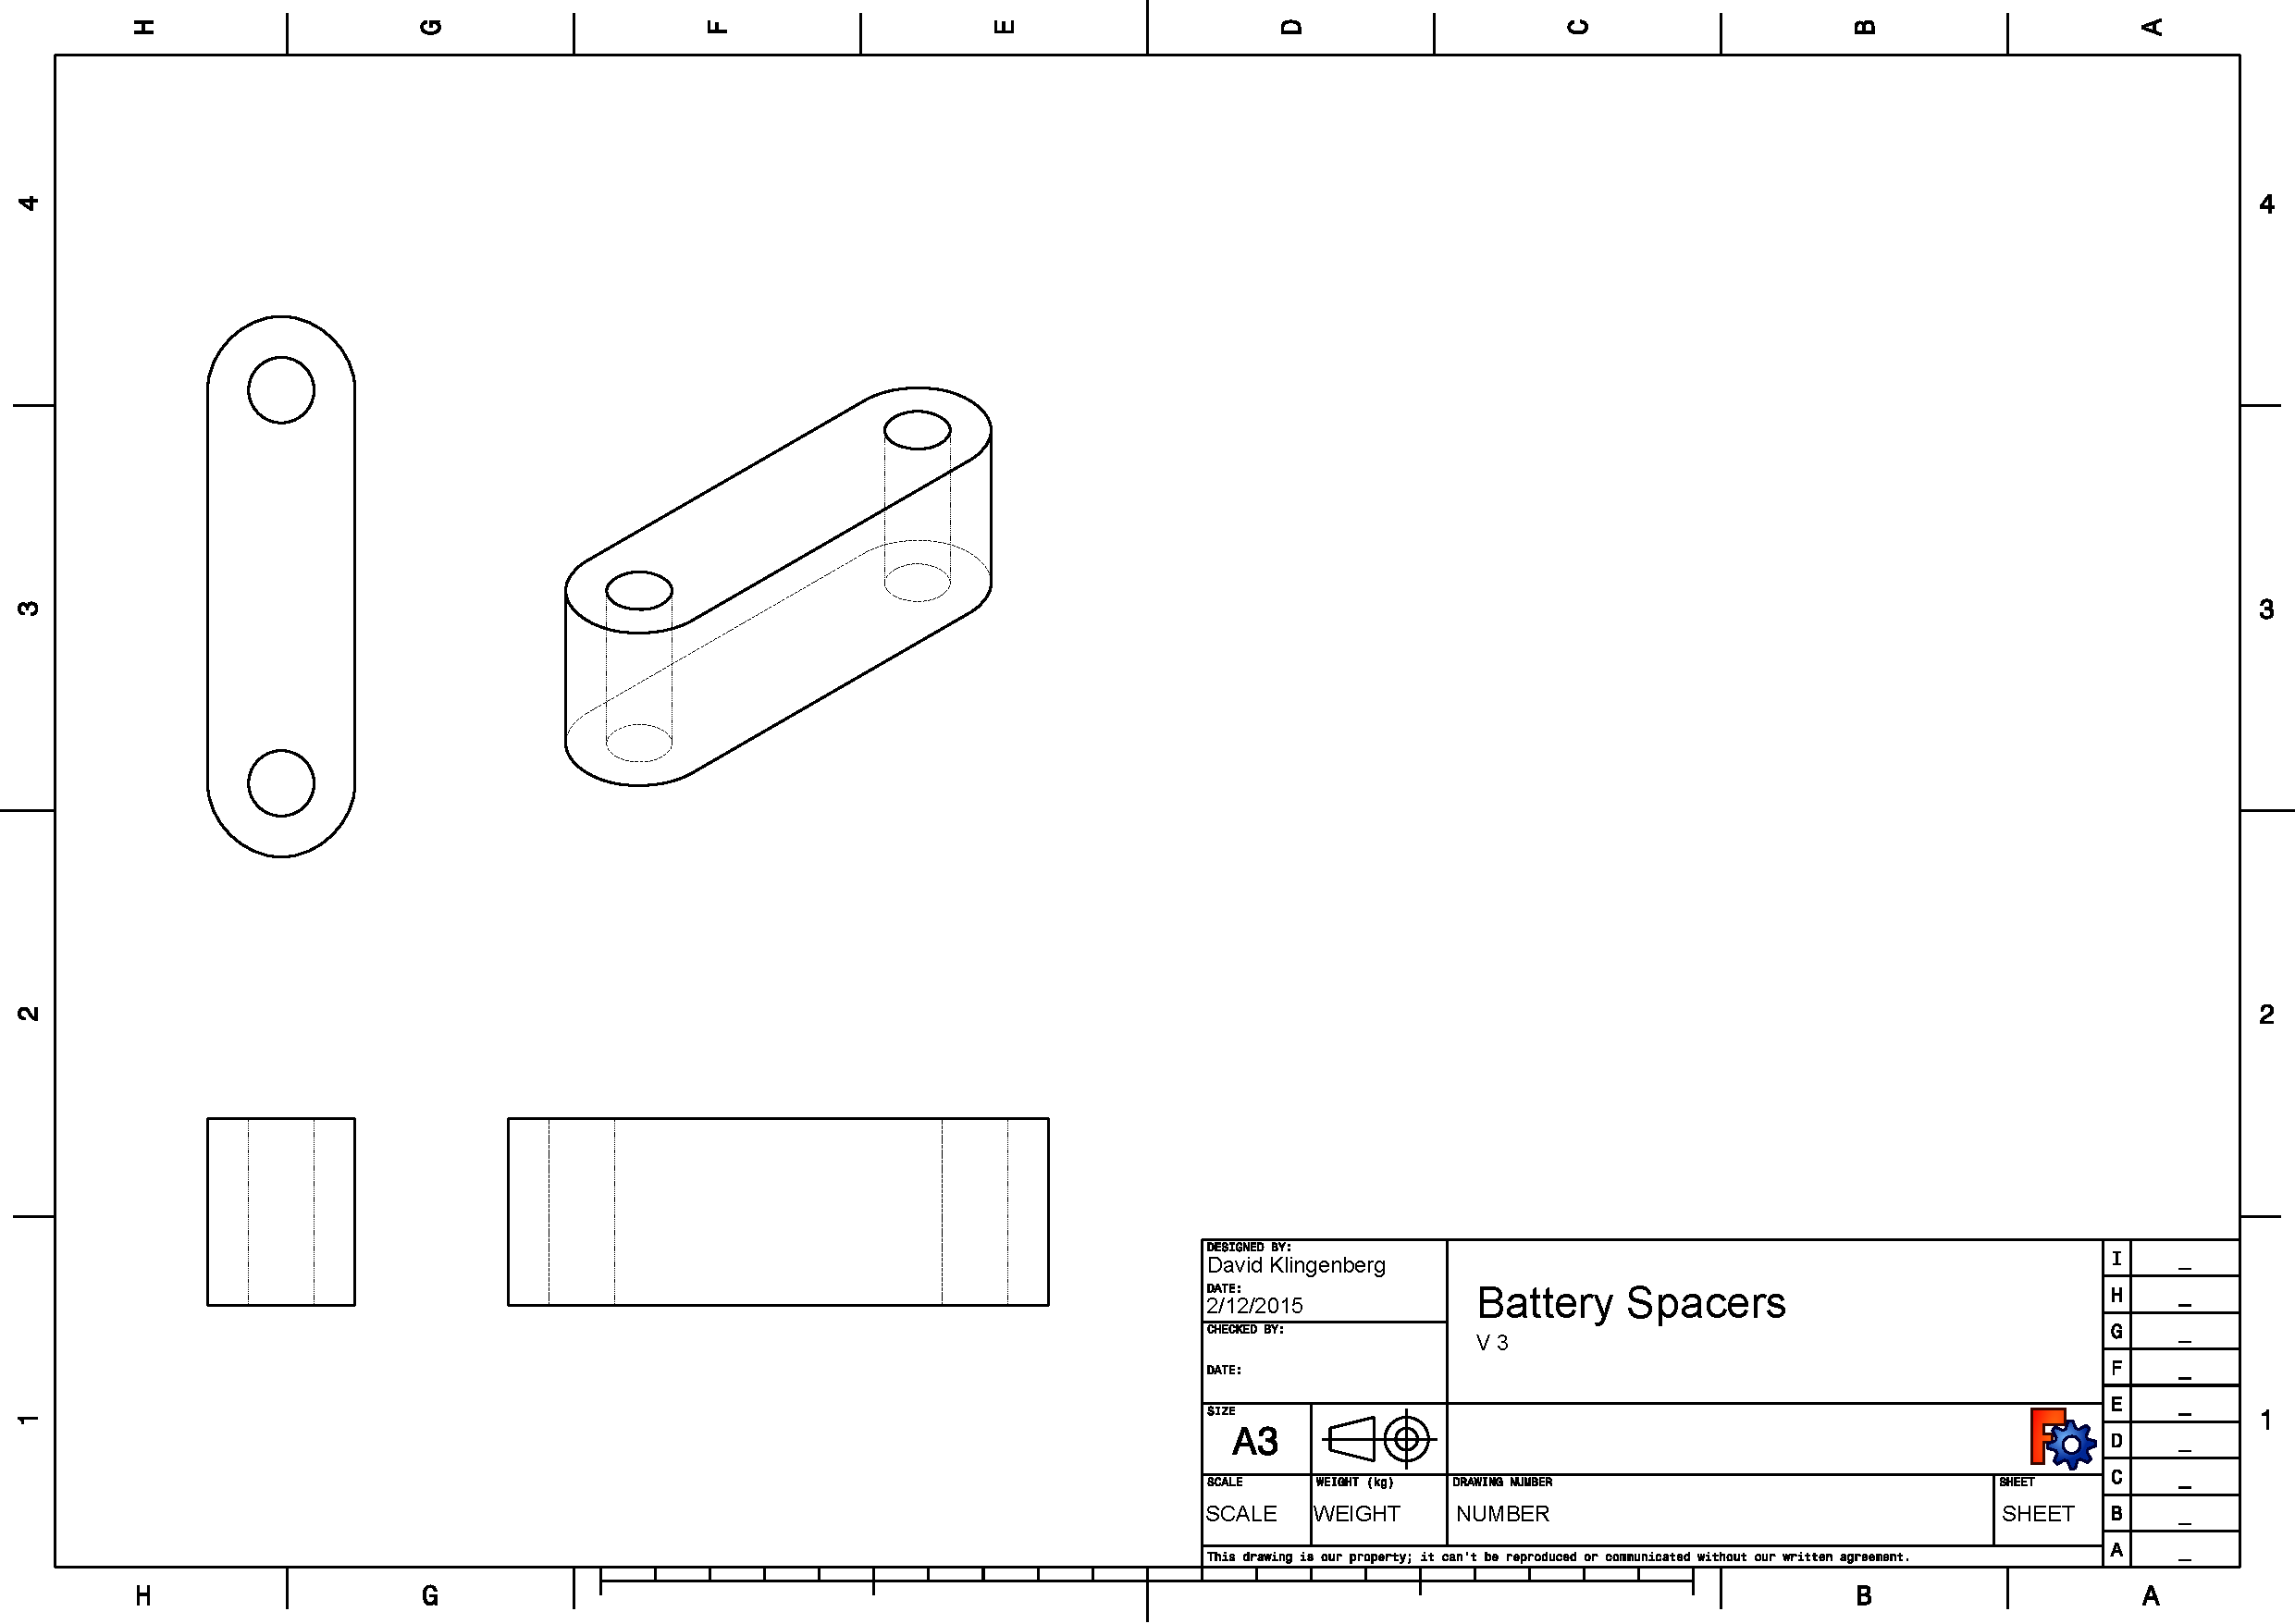
\includegraphics[width=1\textwidth]{./graphics/spacers_battery-eps-converted-to.pdf}
	\caption{Battery Box Spacers}
	\label{fig:batteryspacers}
\end{figure}

\begin{figure}[!h]
	\centering
		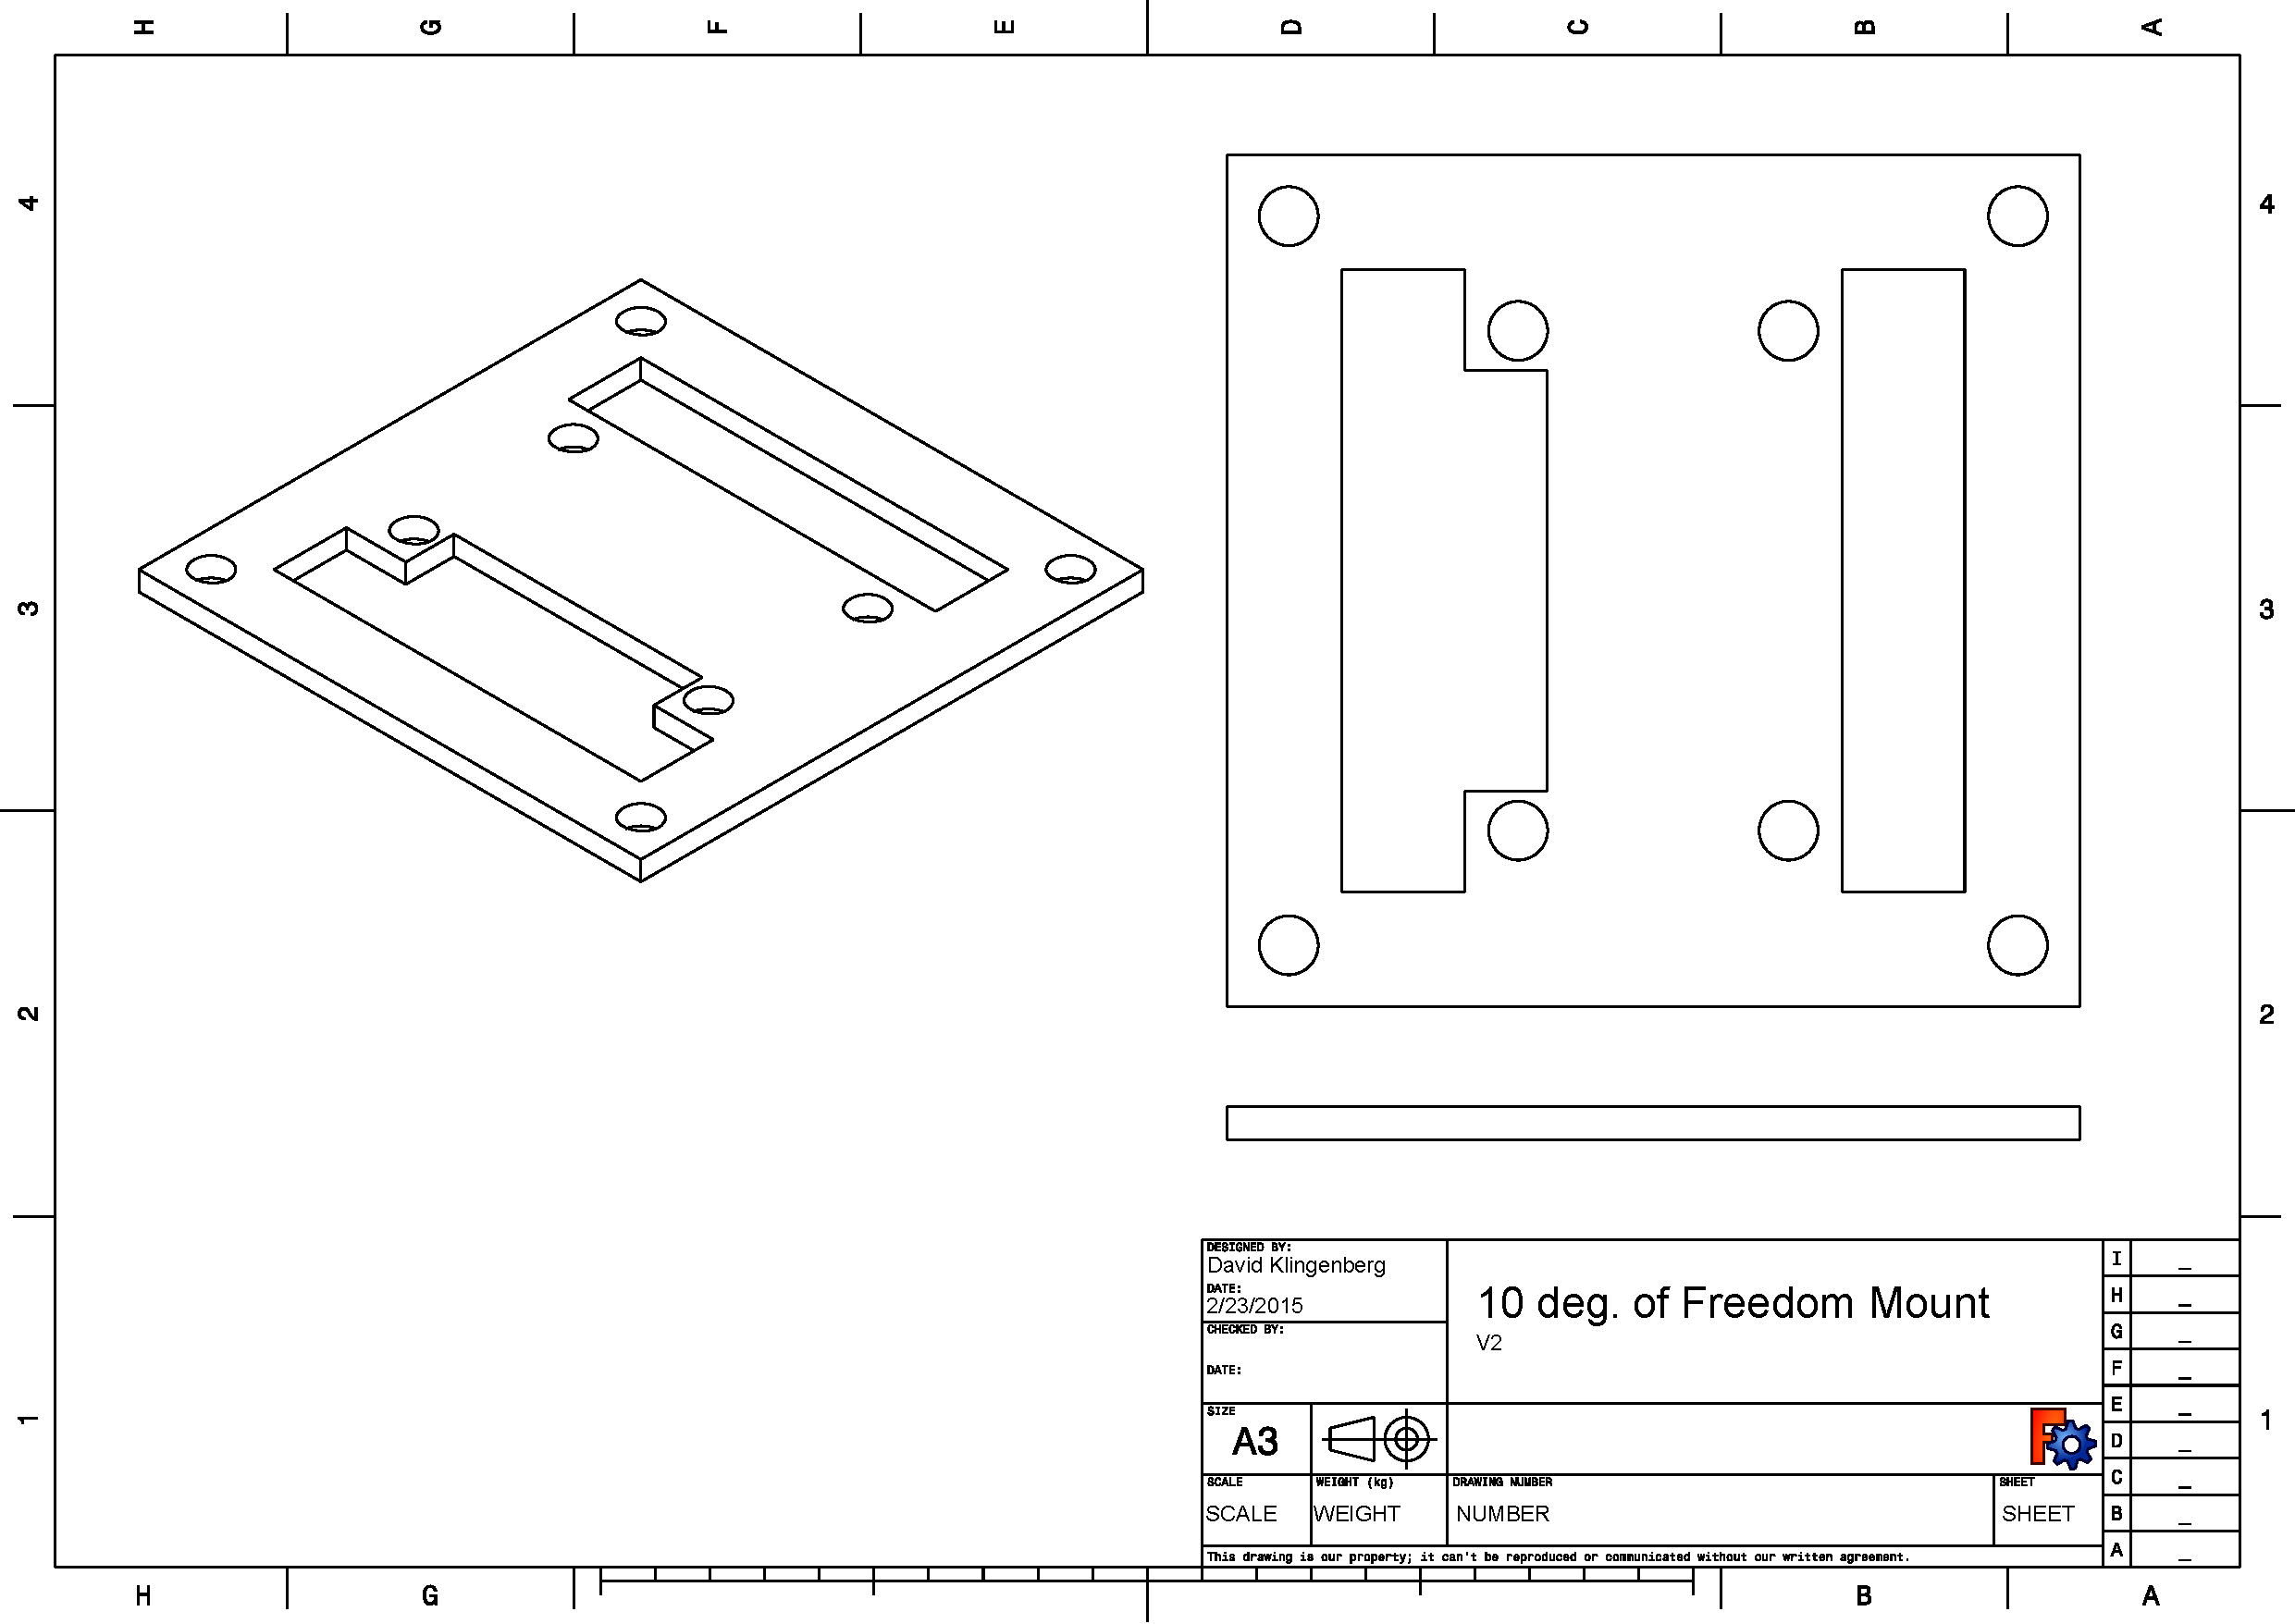
\includegraphics[width=1\textwidth]{./graphics/10_DOF_plate-eps-converted-to.pdf}
	\caption{10 Deg. of Freedom Sensor Platform}
	\label{fig:10freedomplatform}
\end{figure}

\begin{figure}[!h]
	\centering
		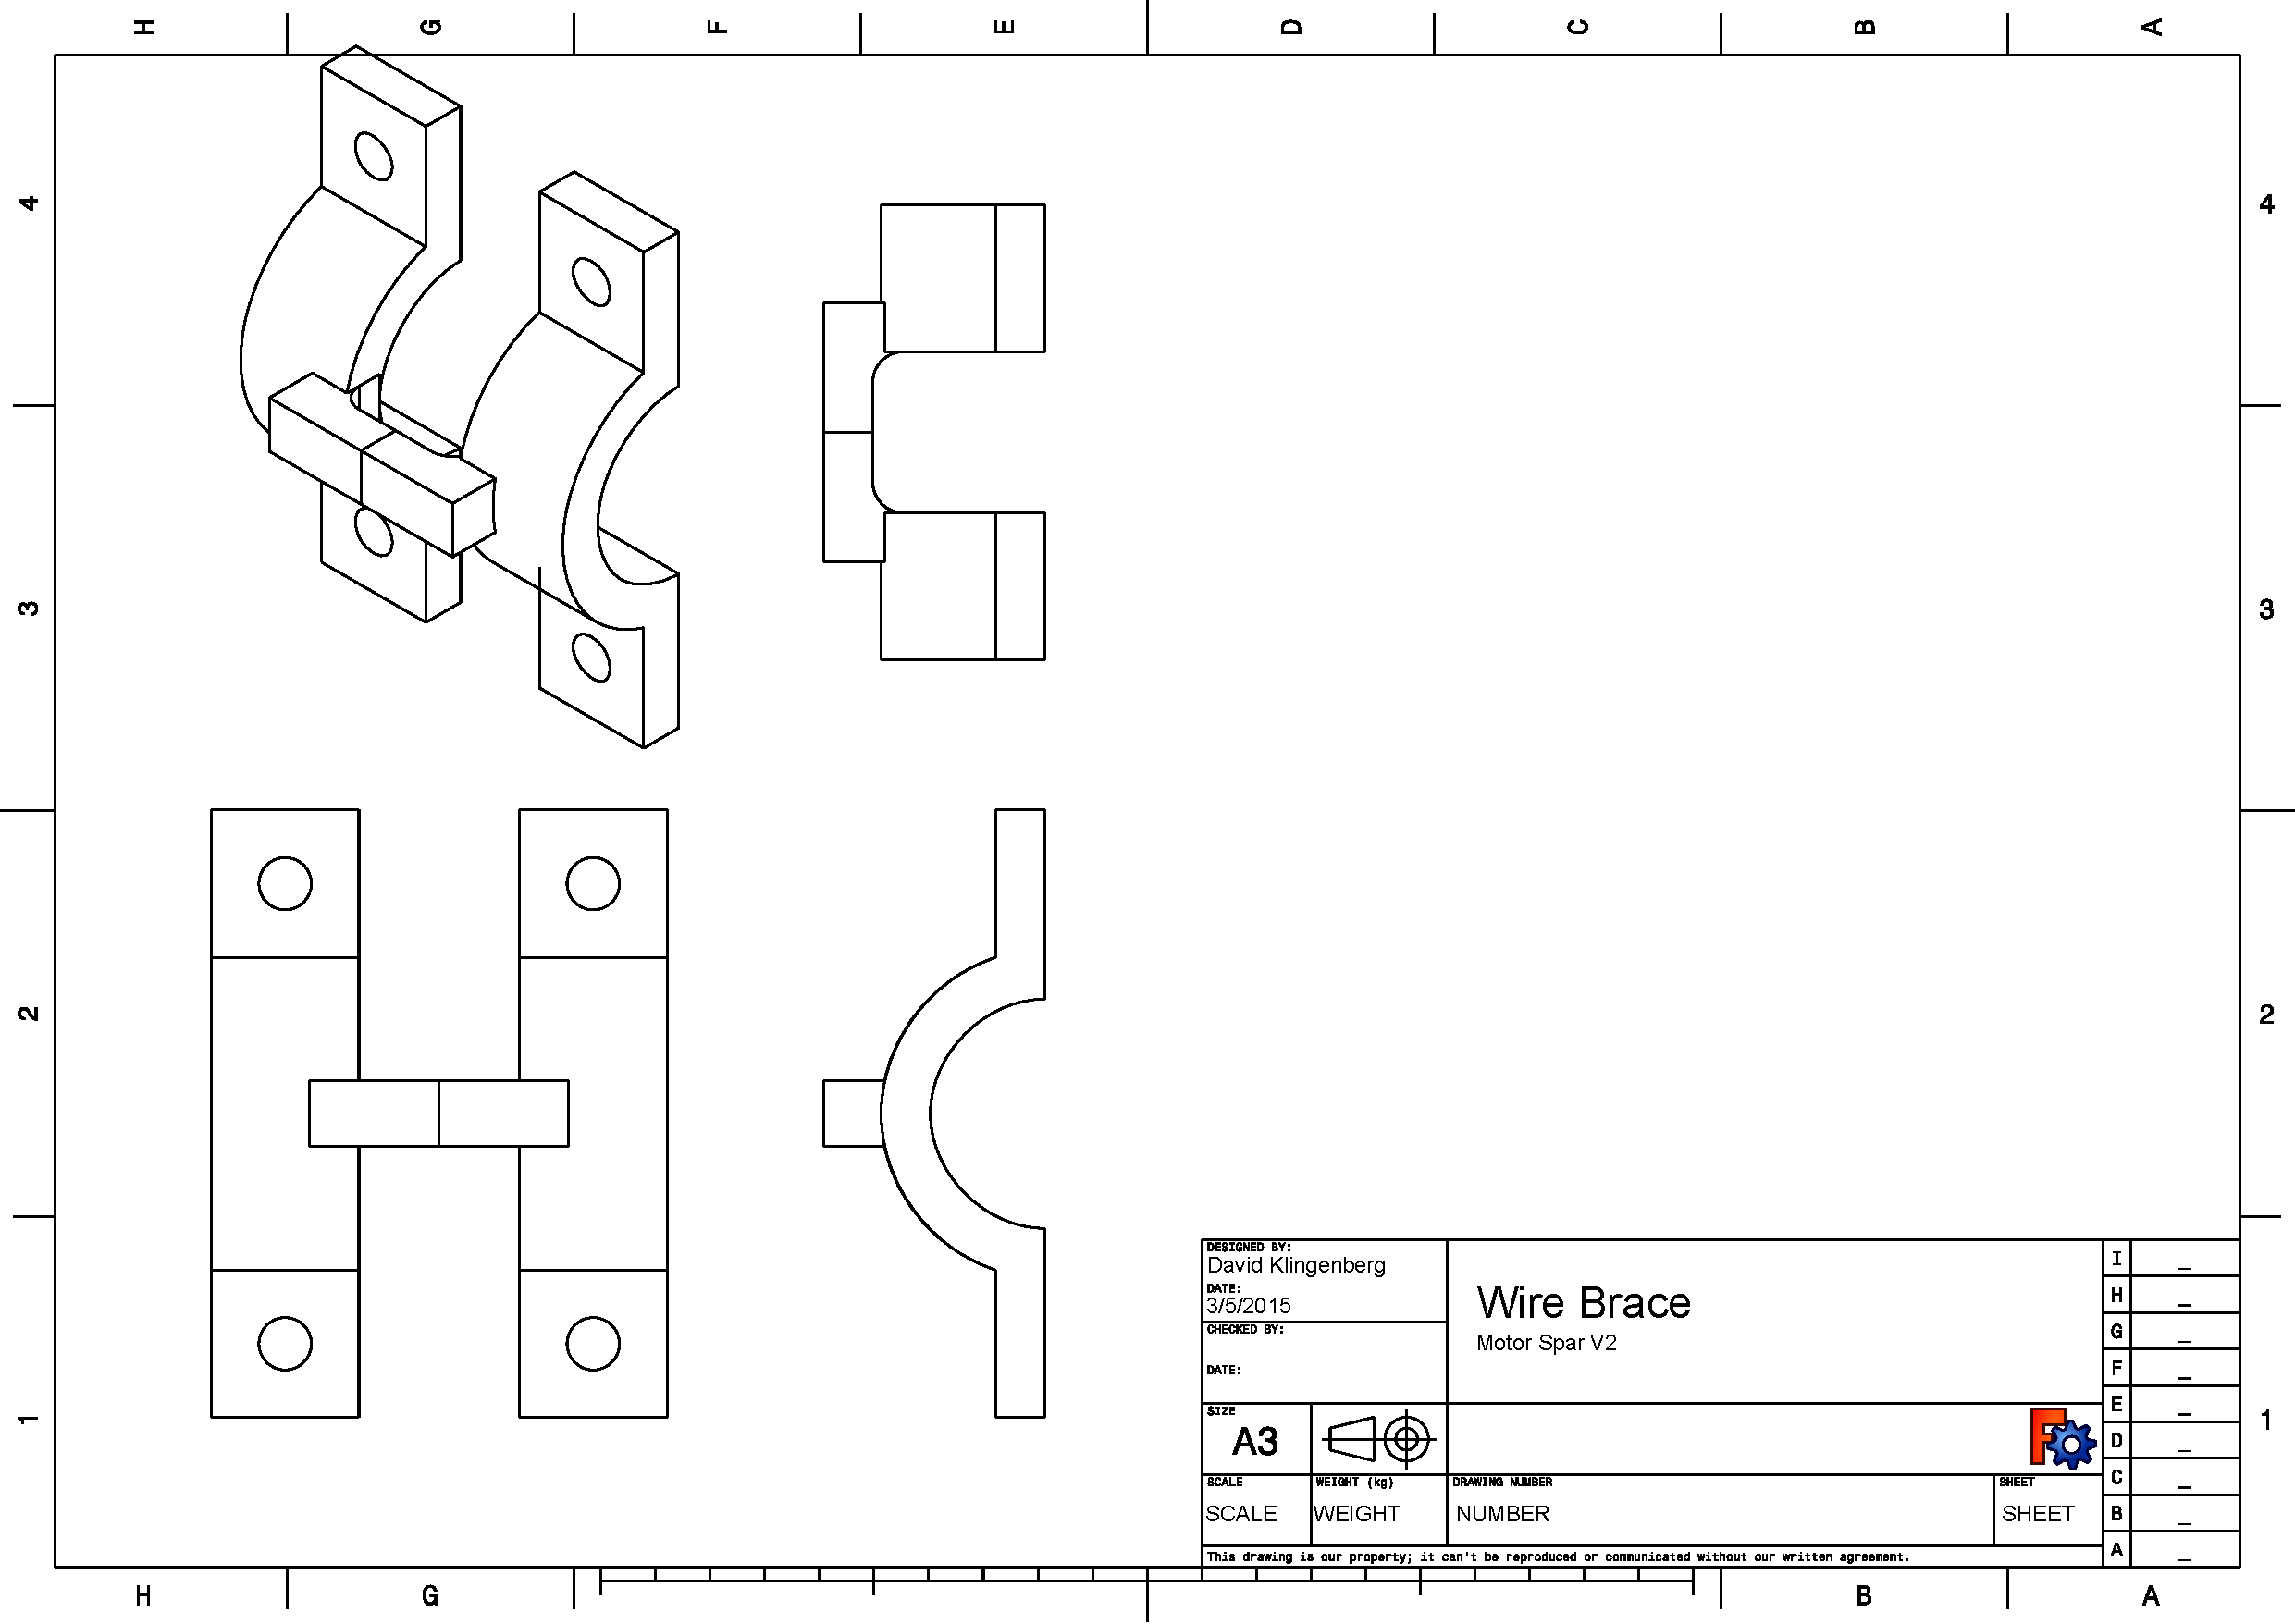
\includegraphics[width=1\textwidth]{./graphics/wire_brace_lowerclamp-eps-converted-to.pdf}
	\caption{Wire Brace}
	\label{fig:wirebrace}
\end{figure}

\begin{figure}[!h]
	\centering
		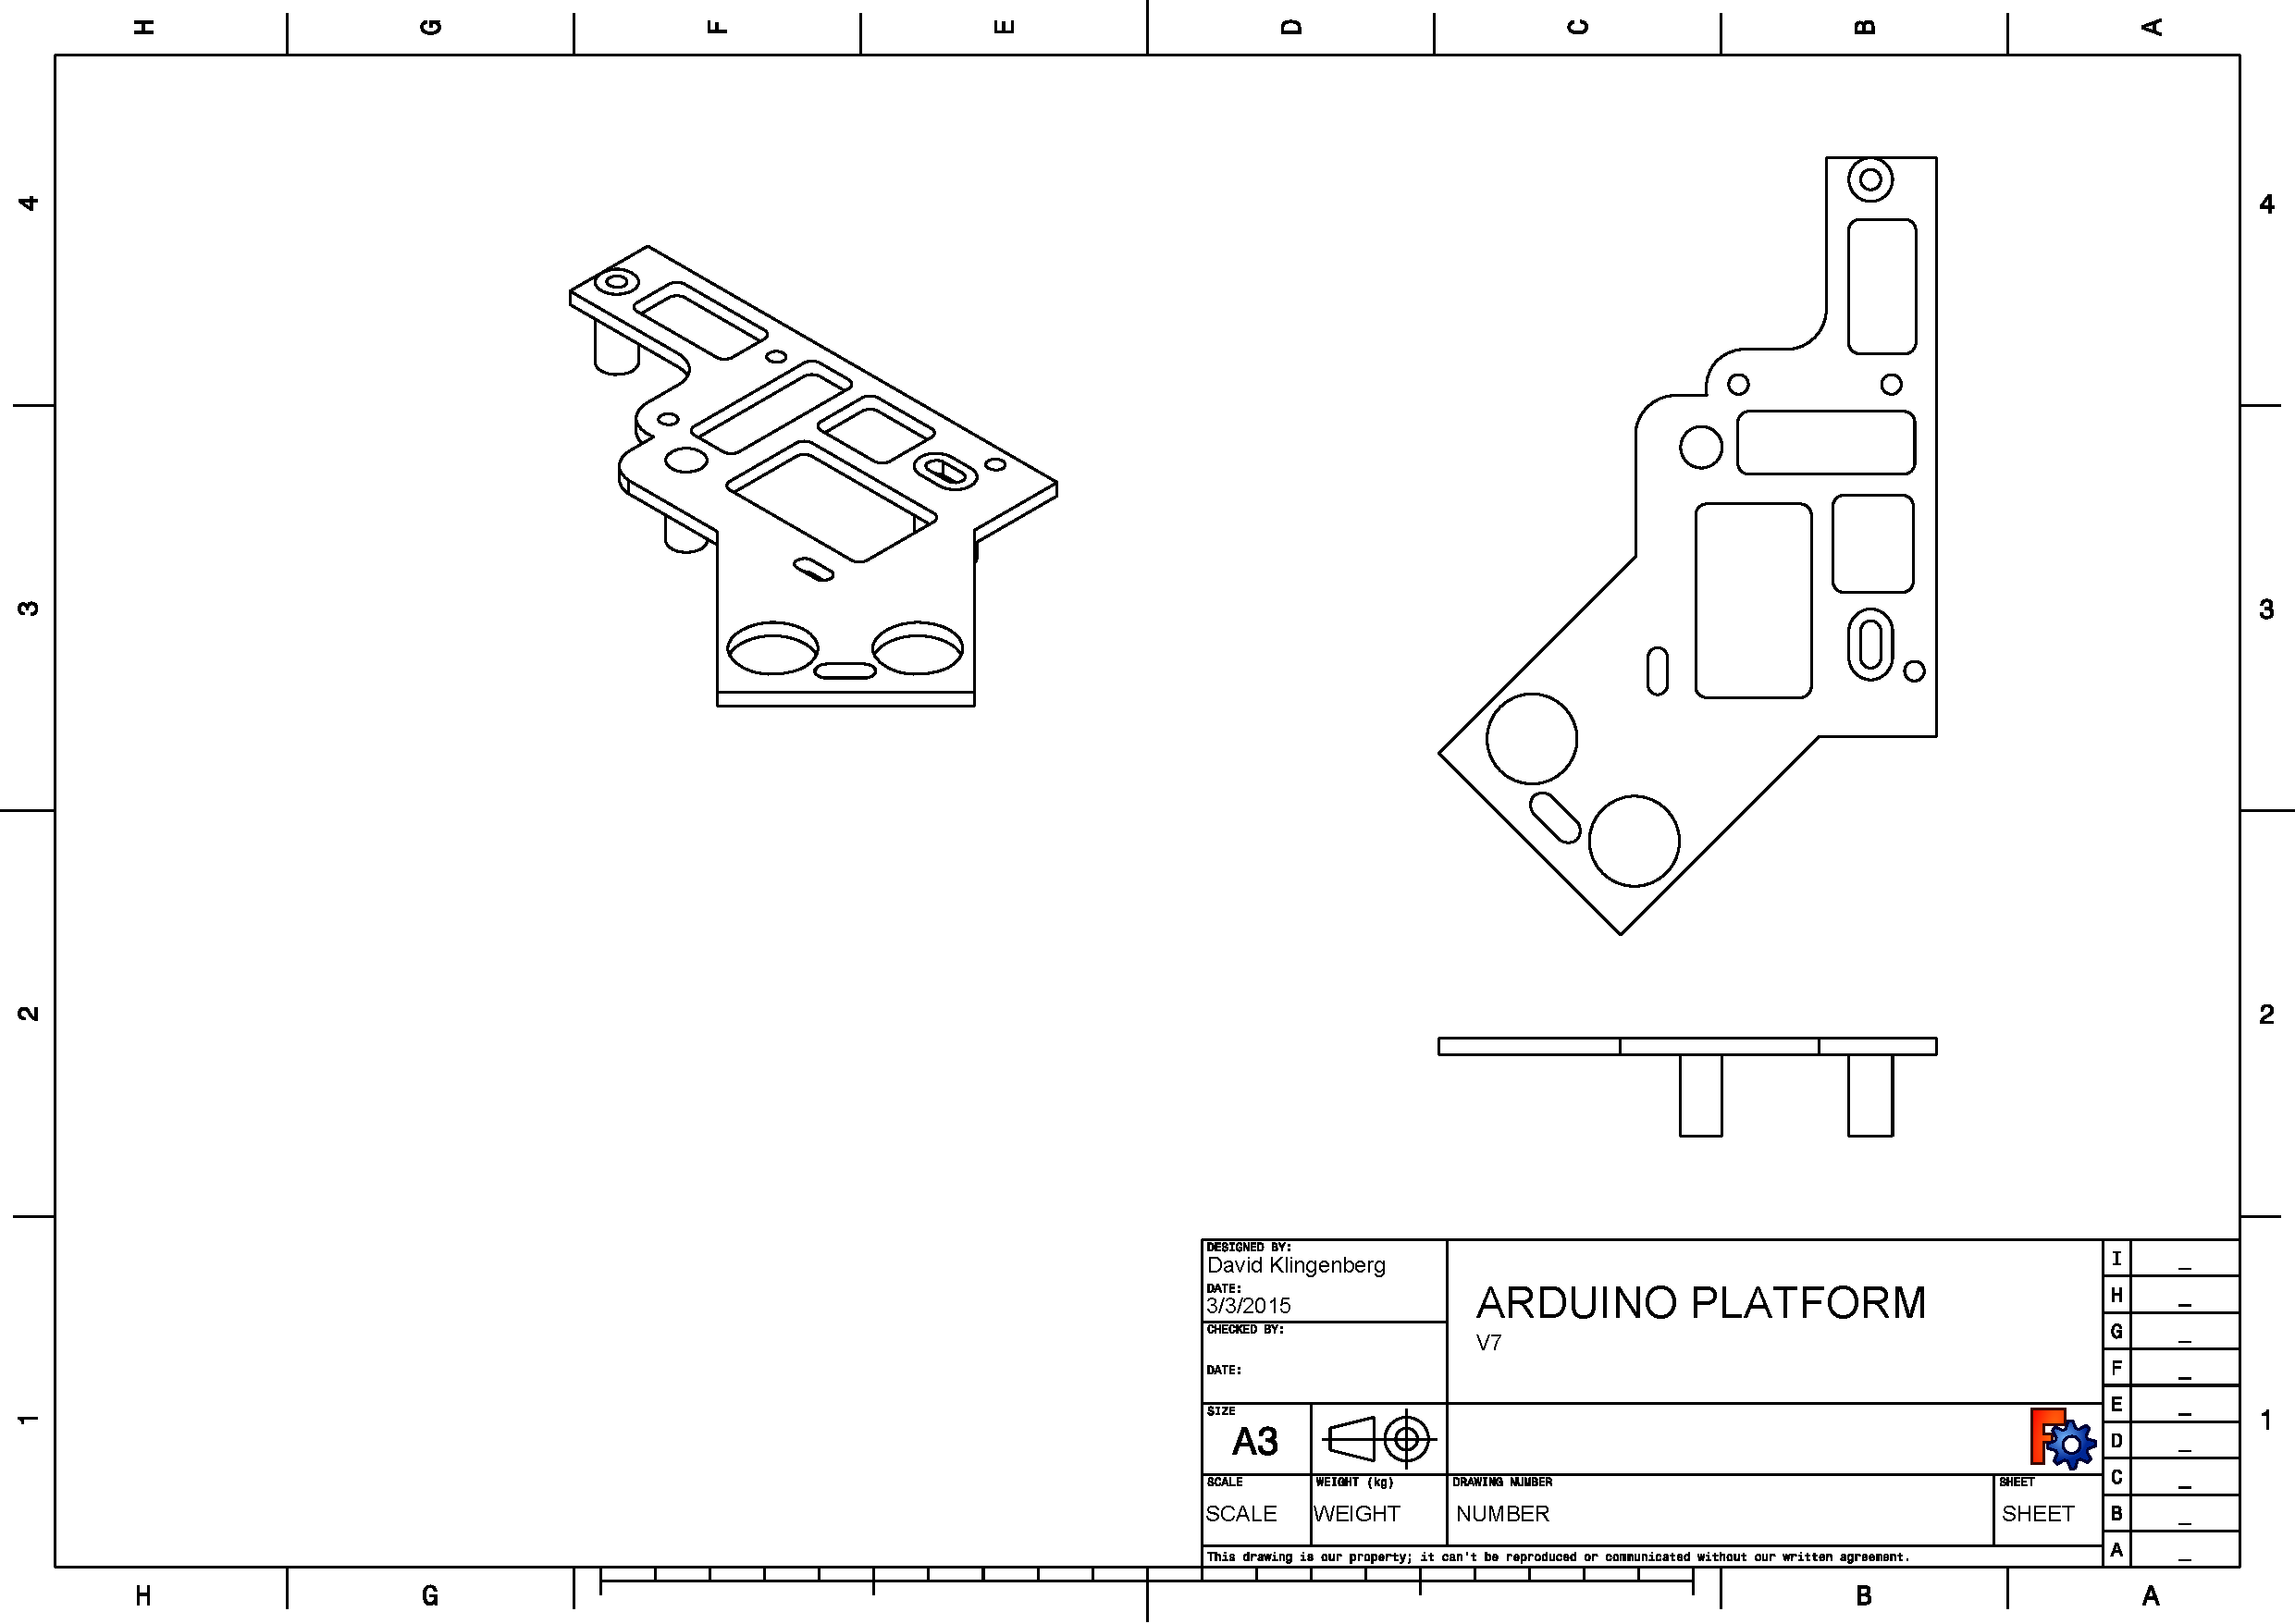
\includegraphics[width=1\textwidth]{./graphics/arduino_platformv7-eps-converted-to.pdf}
	\caption{Arduino Platform}
	\label{fig:arduinoplatform}
\end{figure}

\begin{figure}[!h]
	\centering
		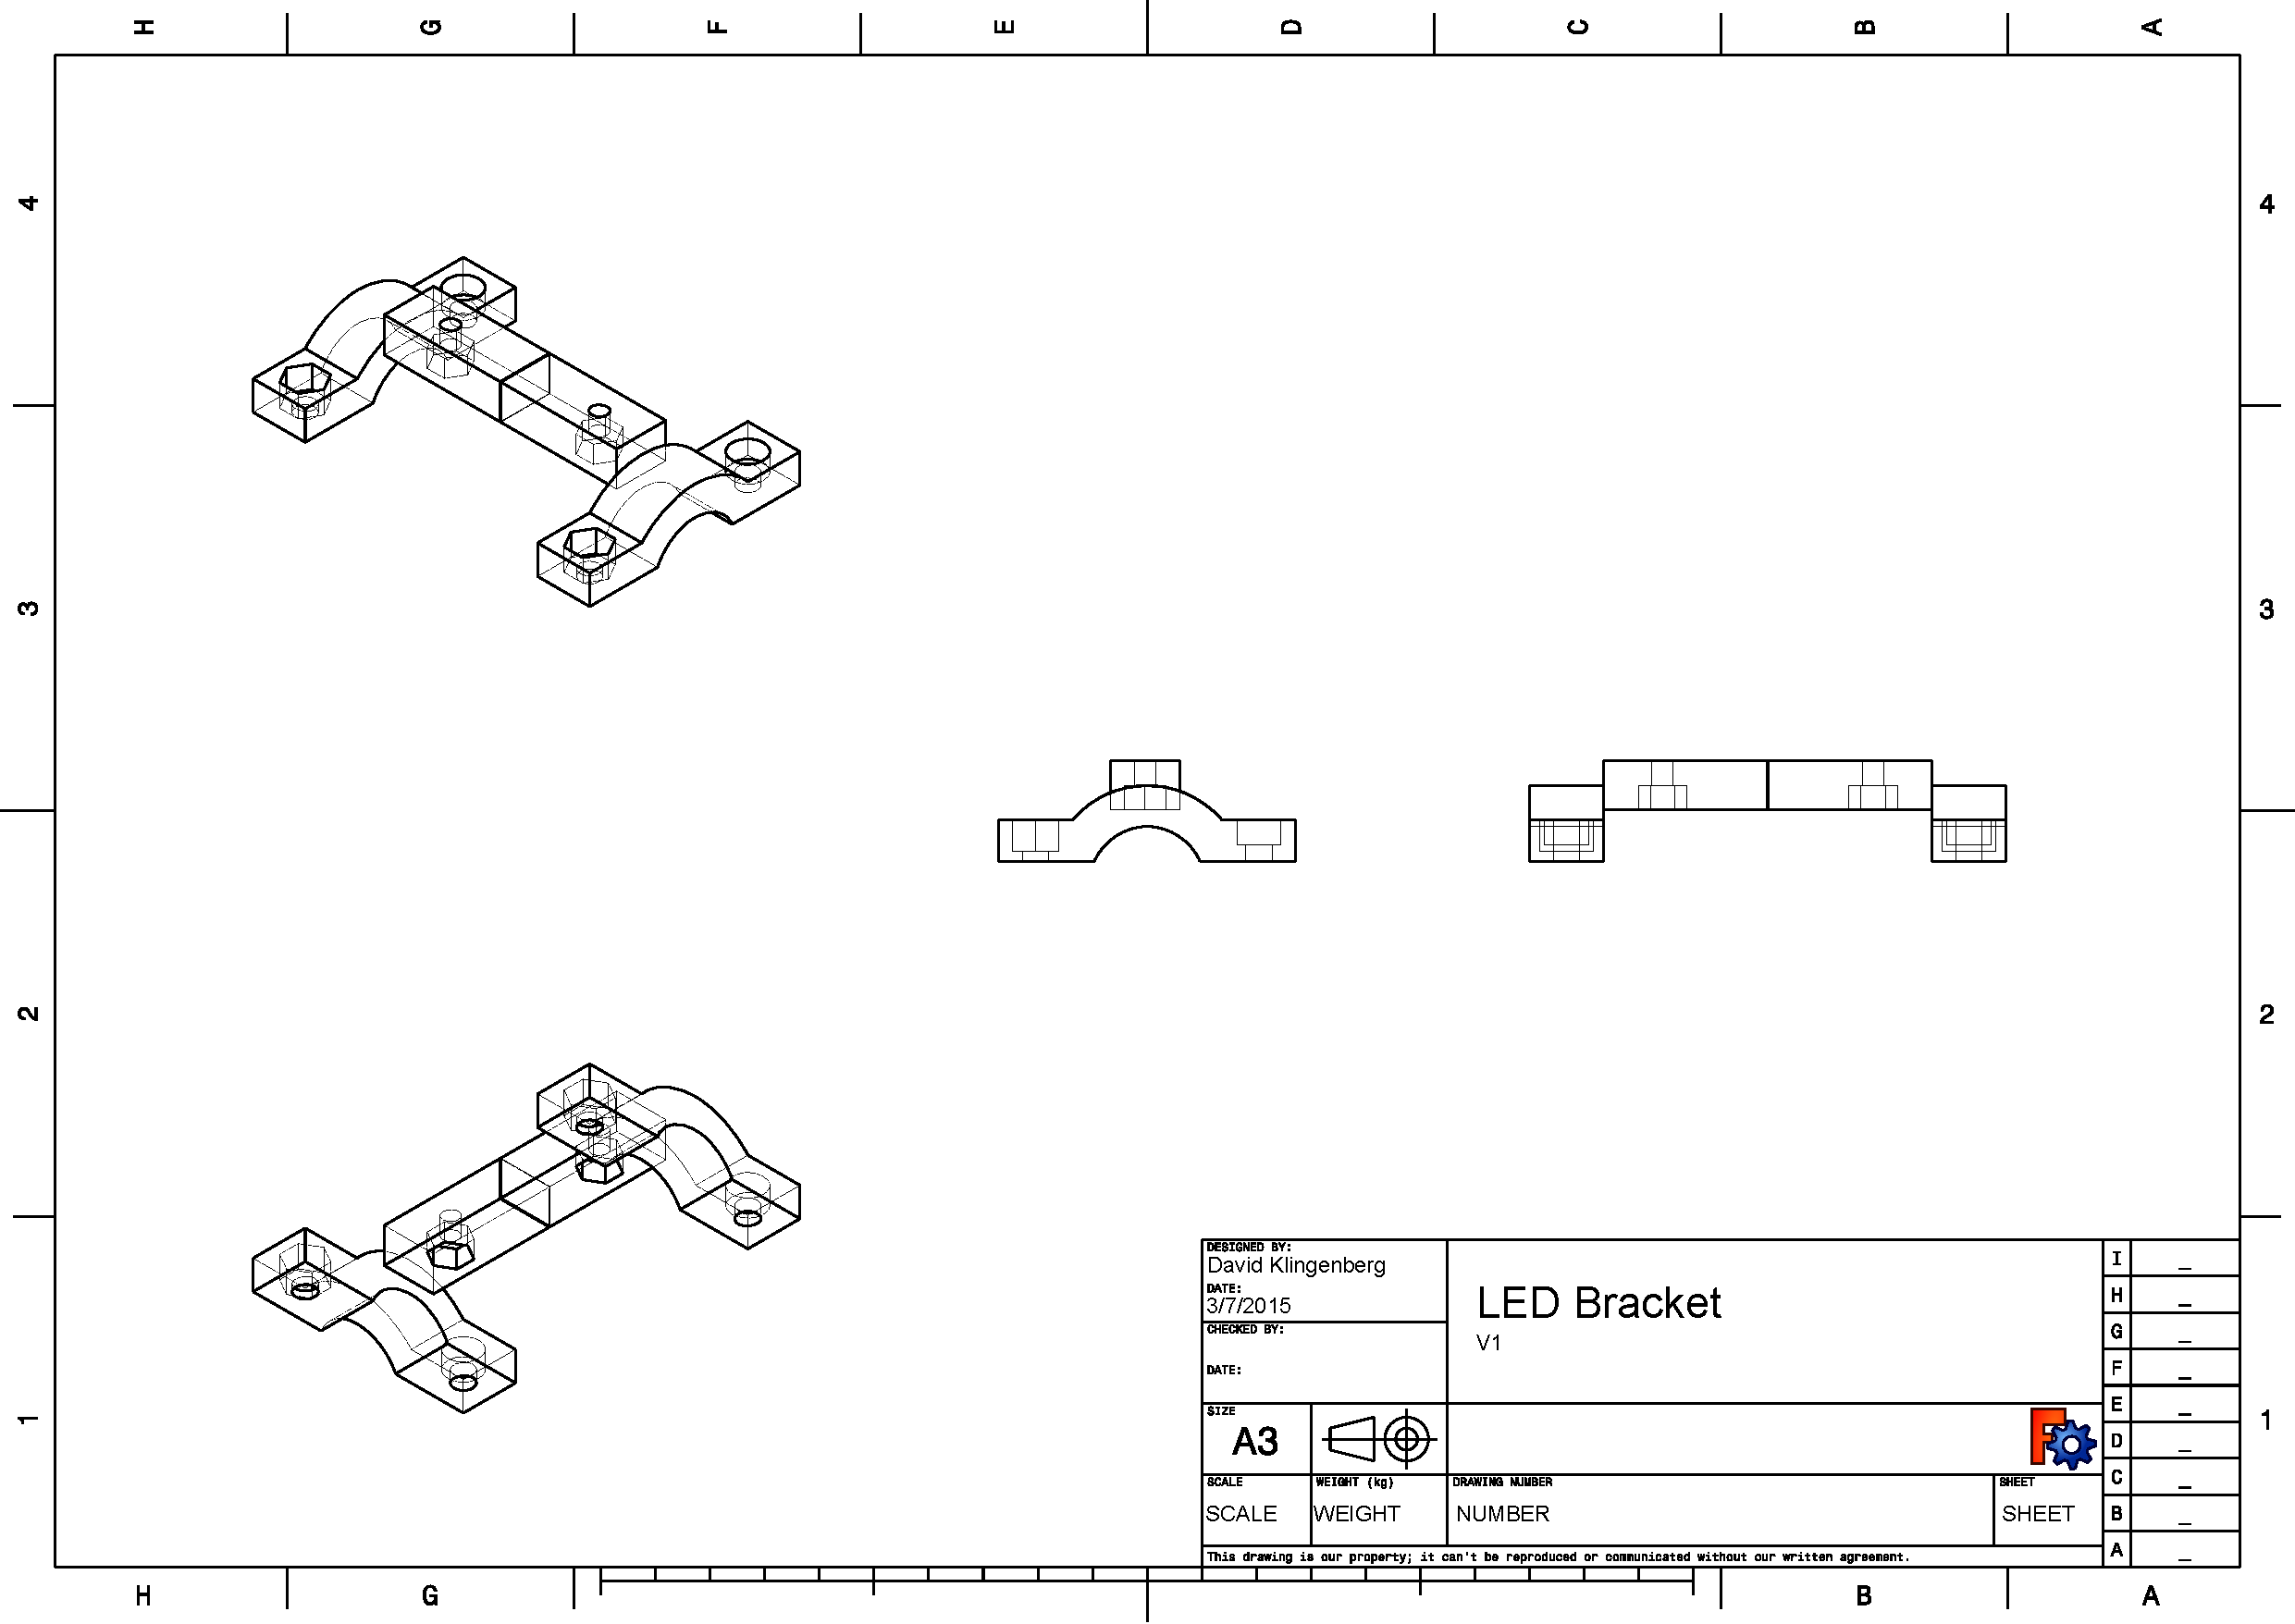
\includegraphics[width=1\textwidth]{./graphics/LED_Bracket-eps-converted-to.pdf}
	\caption{LED Bracket}
	\label{fig:arduinoplatform}
\end{figure}




\end{document}
%%%%%%%%%%%%%%%%%%%%%%%%%%%%%%%%%%%%%%%% END %%%%%%%%%%%%%%%%%%%%%%%%%%%%%%%%%%%%%%%%%%%%%%%%%%